% !TeX root = ../../Book1.tex
% 纲要标题：## 第2章　射影空间、二次曲面与对偶几何
% 纲要位置：几何学计划纲要.md，第 153 行。
% 正文状态：初稿；尚未正式审核。

% 纲要内容开始
% 
% > 本章目标与证明范围：把射影构造、二次对象的分类和极性合成一条连续主线。必须有标准形的存在与唯一性论证，也有由对偶产生的新命题；不把圆锥曲线仅当作公式表。
% 
% 纲要内容结束

\chapter{射影空间、二次曲面与对偶几何}
\label{g1:ch:02}
\BookChapterNumber{g1:ch:02}

\begin{chapterabstract}
	射影空间把仿射位置与无穷远方向放在同一个线性代数模型中。齐次坐标由一维子空间产生，标架固定坐标自由度，交比刻画射影线上的有序四点。二次对象的分类则把上一章的谱定理与惯性定理用于非齐次方程，再经齐次化统一处理实、复射影二次曲面。非退化二次型使点与超平面对应，并把圆锥曲线的六点共线定理转为六条切线的共点定理。最后，通过乘积、二次单项式、子空间与关联条件的坐标模型，看到射影几何如何把一族对象本身组织成新的几何空间。
\end{chapterabstract}

\begin{learninggoals}
	\begin{itemize}
		\item 在齐次坐标与仿射图之间转换，计算子空间的交与张成空间，并用标架和交比确定射影变换。
		\item 对实二次多项式判断中心是否存在，写出 Euclid 、仿射标准形，并说明标准形中哪些数据唯一。
		\item 区分实、复射影二次方程的分类，求曲面所含线性子空间的最大维数，并识别实点集不能保留的信息。
		\item 从配对构造极性，计算切超平面与对偶二次曲面，利用参数与对偶证明圆锥曲线上的构造定理。
		\item 用齐次坐标描述乘积、二次映射和子空间族，检查定义不依赖代表，并从方程恢复原来的几何对象。
	\end{itemize}
\end{learninggoals}

在实平面中，圆 \(x^2+y^2=1\)、双曲线 \(x^2-y^2=1\) 与抛物线 \(y=x^2\) 的外形差别很大。若只允许平移和旋转，这些差别确实无法消除；若还允许改变“哪些点在无穷远处”，情况会怎样？把三个方程分别改写成
\[
	X_1^2+X_2^2=X_0^2,\qquad
	X_1^2-X_2^2=X_0^2,\qquad
	X_1^2=X_0X_2,
\]
并在 \(X_0\ne0\) 时令 \(x=X_1/X_0,y=X_2/X_0\)，原方程便重新出现。而当 \(X_0=0\) 时，三个方程分别没有实射影点、有两个点、有一个点。这提示我们：仿射图中看到的不同形状，有一部分来自二次方程，有一部分来自所选的无穷远直线。

\ProseParagraphBreak

齐次坐标将非零向量的共同缩放归为同一点，使仿射图与无穷远直线可以一起参与坐标变换。二次方程的标准形由此区分方程本身的分类数据与仿射图的选择。随后，二次型的配对 \(B(v,w)\) 会提供一个新的构造：固定一个点的代表 \(v\)，令 \(B(v,w)=0\)，便得到一个超平面。当这个构造可逆时，点的命题可以转成超平面的命题；在平面中，共线与共点由此相互对应。

\ProseParagraphBreak

本章实际使用的线性代数包括基、秩与核、对偶空间，以及实对称矩阵的两种标准形。其中\cref{g1:thm:spectral}要求实内积与正交换基，保留特征值；\cref{g1:thm:inertia}允许一般实换基，保留正、负、零三个维数。两种结果的区别会在分类中反复出现，所需条件将在调用处恢复。切线与切超平面由二次方程的一次变化直接计算。射影空间、标架、交比与对偶的补充阅读可参看 Gallier 的正式第二版\cite[第5.2--5.9, 5.11节]{Gallier2011Geometric}。

% !TeX root = ../../Book1.tex
% 纲要标题：### 2.1 从仿射图到射影空间
% 纲要位置：几何学计划纲要.md，第 157 行。
% 正文状态：初稿；尚未正式审核。

% 纲要内容开始
% 
% * 一维子空间、齐次坐标与标准仿射图
% * 射影子空间的关联与维数
% * 射影标架及射影变换的唯一确定
% * 射影线上的交比与置换对称
% 
% 纲要内容结束

\section{从仿射图到射影空间}
\label{g1:sec:0201}

在仿射平面中，两条不同直线的关系要分成相交与平行两种。可是从透视图看，平行铁轨似乎也交于远方。射影空间把这种现象变成一个精确的构造：把方向也作为点加入，使平面内任意两条不同直线都有唯一交点。这些方向点将由向量的一维子空间来定义。

\subsection{一维子空间、齐次坐标与标准仿射图}
\label{g1:subsec:0201:01}

本章的基域 \(K\) 为 \(\mathbb R\) 或 \(\mathbb C\)。上一章的仿射组合、基与维数计算也可对复向量空间逐字进行；长度、正负号与正交分类则仍须注明是实 Euclid 结构，不能随之自动推广。

\begin{definition}[射影空间]\label{g1:def:projective-space}
	设 \(K=\mathbb R\) 或 \(\mathbb C\)，\(V\) 是 \(n+1\) 维 \(K\) 向量空间，\(n\geq0\)。以 \(V\) 的一维向量子空间为元素的集合
	\[
		\mathbb P(V)\coloneqq\{Kv:v\in V\setminus\{0\}\}
	\]
	称为 \(V\) 的\term[sheyingkongjian]{射影空间}[projective space]，其射影维数定义为 \(n\)。记 \([v]=Kv\)，并记 \(\mathbb P^n(K)=\mathbb P(K^{n+1})\)。选定 \(V\) 的基后，若 \(v=(X_0,\ldots,X_n)\ne0\)，则 \([X_0:\cdots:X_n]\) 称为该点的\term[qicizuobiao]{齐次坐标}[homogeneous coordinates]。
\end{definition}
\symidx{\(\mathbb P(V)\)：向量空间的一维子空间所成的射影空间}

两个非零向量表示同一点，当且仅当相差一个非零倍数：
\[
	[X_0:\cdots:X_n]=[\lambda X_0:\cdots:\lambda X_n]\qquad(\lambda\in K^\times).
\]
零向量不表示任何射影点。在实数情形，\(v\) 与 \(-v\) 也表示同一点，所以这里取的是过原点的整条直线，并非带方向的射线。\(\mathbb P^0(K)\) 只有一个点，而 \(\mathbb P^1(K)\) 已有无穷多个点。

\begin{proposition}[标准仿射图]\label{g1:prop:projective-charts}
	设 \(K=\mathbb R\) 或 \(\mathbb C\)。对 \(0\leq i\leq n\)，令
	\[
		U_i=\{[X_0:\cdots:X_n]:X_i\ne0\}.
	\]
	映射 \(U_i\rightarrow K^n\) 将一点送到除去第 \(i\) 项后的各个比值 \(X_j/X_i\)，是双射。这些集合覆盖 \(\mathbb P^n(K)\)。在 \(U_i\cap U_k\) 上，若 \(x_j=X_j/X_i\)，并补记 \(x_i=1\)，则第 \(k\) 张图的坐标为 \(y_j=x_j/x_k\)，其中 \(j\ne k\)。
\end{proposition}
\begin{proof}
	同乘非零数不改变任何比值，故映射良定义。反过来，把第 \(i\) 项取为 \(1\)，其余项依次取为所给的 \(n\) 个数，便得到唯一射影点。每个非零向量至少有一个非零分量，所以各图覆盖整个空间。在重叠处 \(x_k\ne0\)，直接相除给出 \(X_j/X_k=(X_j/X_i)/(X_k/X_i)\)，即所述换图公式。
\end{proof}

称 \(U_i\) 为\term[fangshetu]{仿射图}[affine chart]，因为选定归一化 \(X_i=1\) 后它具有通常的仿射坐标。不同图的换图映射一般不是仿射映射。例如在射影线上，\(t=X_0/X_1\) 与 \(s=X_1/X_0\) 满足 \(s=1/t\)。图的用途是让我们在一块区域内使用熟悉的坐标，并明确知道走到另一块区域时如何转换。

\begin{example}[一条射影线中的无穷远点]\label{g1:exm:projective-line}
	在 \(\mathbb P^1(K)\) 中，\(U_1\) 的点唯一写成 \([t:1]\)，余下只有 \([1:0]\)，记作 \(\infty\)。因此作为集合有 \(\mathbb P^1(K)=K\cup\{\infty\}\)。这里的记号不允许直接参与普通实数或复数运算；例如涉及 \(\infty\) 的分式应改用齐次坐标计算。在实数情形，\cref{g1:fig:projective-line-chart}用穿过原点的直线表示这些点。
\end{example}

\begin{figure}[htbp]
	\centering
	% !TeX root = ../Book1.tex
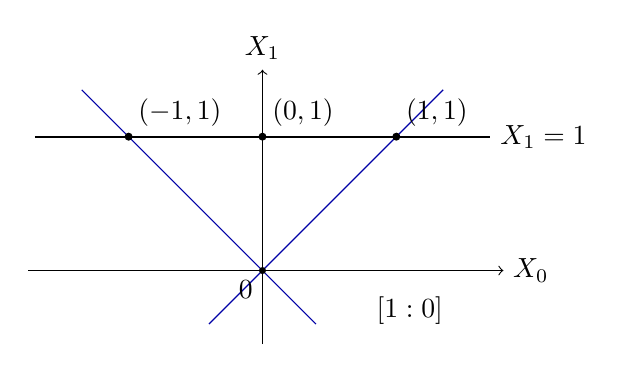
\begin{tikzpicture}[scale=0.85]
	\draw[->] (-3.5,0)--(3.6,0) node[right] {\(X_0\)};
	\draw[->] (0,-1.1)--(0,3) node[above] {\(X_1\)};
	\draw[thick] (-3.4,2)--(3.4,2) node[right] {\(X_1=1\)};
	\draw[blue!65!black] (-0.8,-0.8)--(2.7,2.7);
	\draw[blue!65!black] (0.8,-0.8)--(-2.7,2.7);
	\fill (0,0) circle(1.5pt) node[below left] {\(0\)};
	\foreach \x/\lab in {-2/{(-1,1)},0/{(0,1)},2/{(1,1)}}
	{\fill (\x,2) circle(1.7pt);\node[above right] at (\x,2) {\(\lab\)};}
	\node[below] at (2.2,-0.25) {\([1:0]\)};
\end{tikzpicture}

	\caption[射影线与一张仿射图]{射影线与一张仿射图。与 \(X_1=1\) 相交的每条过原点直线给出一个有限坐标；水平直线 \(X_1=0\) 给出唯一遗漏的射影点 \([1:0]\)。}
	\label{g1:fig:projective-line-chart}
\end{figure}

对 \(\mathbb P^n(K)\)，其中 \(n\geq1\)，选取 \(U_0\)，便把 \(K^n\) 放入射影空间：
\[
	(x_1,\ldots,x_n)\longmapsto[1:x_1:\cdots:x_n].
\]
补集 \(H_\infty=\{X_0=0\}\cong\mathbb P^{n-1}(K)\) 称为这张图的\term[wuqiongyuanchaopingmian]{无穷远超平面}[hyperplane at infinity]。它取决于仿射图的选择，并不是射影空间中预先指定的特殊部分。当 \(n=1\) 时它是一个点；当 \(n=2\) 时是一条射影直线。

\subsection{射影子空间的关联与维数}
\label{g1:subsec:0201:02}

由线性方程定义子空间的办法仍然适用，不过现在方程必须齐次，才能使“是否满足方程”不依赖代表向量。

\begin{definition}[射影子空间]\label{g1:def:projective-subspace}
	设 \(K=\mathbb R\) 或 \(\mathbb C\)，\(V\) 为有限维 \(K\) 向量空间。若 \(W\subseteq V\) 为非零向量子空间，称 \(\mathbb P(W)\subseteq\mathbb P(V)\) 为\term[sheyingzikongjian]{射影子空间}[projective subspace]，维数为 \(\dim_K W-1\)。维数为 \(1\) 的称为\term[sheyingzhixian]{射影直线}[projective line]；余维为 \(1\) 的称为\term[sheyingchaopingmian]{射影超平面}[projective hyperplane]。为统一相交公式，也把空集视为空射影子空间，约定 \(\mathbb P(0)=\varnothing\)，\(\dim\varnothing=-1\)。
\end{definition}

\begin{proposition}[交与张成空间]\label{g1:prop:projective-dimension}
	设 \(K=\mathbb R\) 或 \(\mathbb C\)，\(V\) 为有限维 \(K\) 向量空间，\(U,W\subseteq V\) 为向量子空间，记 \(E=\mathbb P(U)\)、\(F=\mathbb P(W)\)，并约定空射影子空间的维数为 \(-1\)。则 \(\mathbb P(U)\cap\mathbb P(W)=\mathbb P(U\cap W)\)，包含二者的最小射影子空间为 \(\mathbb P(U+W)\)，称为它们的张成空间。若用 \(\langle E,F\rangle\) 表示两个射影子空间的张成空间，则
	\[
		\dim\langle E,F\rangle+\dim(E\cap F)=\dim E+\dim F.
	\]
	特别地，在 \(\mathbb P^n(K)\) 中，\(\dim E+\dim F\geq n\) 蕴含 \(E\cap F\ne\varnothing\)。
\end{proposition}
\begin{proof}
	一个一维空间同时包含于 \(U,W\)，等价于它包含于 \(U\cap W\)，故得交集公式。任何包含 \(\mathbb P(U),\mathbb P(W)\) 的射影子空间，其对应向量空间包含 \(U,W\)，因而包含 \(U+W\)；后者本身也满足包含要求，故为最小者。上一章证明\cref{g1:prop:affine-intersection}时已经通过扩充交集的基得到 \(\dim(U+W)+\dim(U\cap W)=\dim U+\dim W\)。四个维数各减 \(1\)，即得到此处公式，零空间也符合约定。若交集为空，公式给出 \(\dim\langle E,F\rangle=\dim E+\dim F+1\leq n\)，与最后的假设矛盾。
\end{proof}

所以射影平面中两条不同直线恰交于一点：必有交点，而若交空间维数至少为 \(1\)，两条直线就相同。但射影三维空间仍有不相交的直线。例如 \(\mathbb P(\operatorname{span}(e_0,e_1))\) 与 \(\mathbb P(\operatorname{span}(e_2,e_3))\) 不交。加入无穷远点消除了平面内平行线的例外，没有消除高维空间中的异面直线。

\begin{proposition}[仿射子空间的射影补全]\label{g1:prop:affine-projective-completion}
	设 \(K=\mathbb R\) 或 \(\mathbb C\)，\(n\geq1\)，\(F=p+L\subseteq K^n\) 为非空仿射子空间，\(\dim L=d\)。用 \(x\mapsto[1:x]\) 把 \(K^n\) 识别为 \(U_0=\{X_0\ne0\}\subseteq\mathbb P^n(K)\)，并记 \(H_\infty=\{X_0=0\}\)。在此嵌入下，包含 \(F\) 的最小射影子空间为
	\[
		\widehat F=\mathbb P\bigl(K(1,p)+(0,L)\bigr).
	\]
	它具有维数 \(d\)，与 \(U_0\) 的交为 \(F\)，与 \(H_\infty\) 的交为 \(\mathbb P(0,L)\)。
\end{proposition}
\begin{proof}
	所写向量空间包含所有 \((1,p+u)=(1,p)+(0,u)\)，其中 \(u\in L\)。反过来，任何包含这些向量所张成各条直线的向量空间都含 \((1,p)\)，再作差便含全部 \((0,u)\)，故包含所写空间。由于 \((1,p)\notin(0,L)\)，其向量维数为 \(d+1\)。一般向量为 \((a,ap+u)\)：若 \(a\ne0\)，归一化得到 \([1:p+u/a]\)；若 \(a=0\)，得到 \([0:u]\)。这分别给出两种交集。
\end{proof}

\begin{example}[平行线的公共方向点]\label{g1:exm:parallel-infinity}
	在实仿射平面中，两条直线 \(y=0\)、\(y=1\) 的射影补全分别为 \(X_2=0\)、\(X_2=X_0\)。联立可得唯一交点 \([0:1:0]\)，它代表水平方向。一般地，不同平行直线 \(p+Ku\)、\(q+Ku\) 的射影补全都含 \([0:u]\)，而有限部分不交，故交点恰是该方向点。
\end{example}

\subsection{射影标架及射影变换的唯一确定}
\label{g1:subsec:0201:03}

上一章的仿射标架由 \(n+1\) 个点构成，它们唯一确定仿射映射。在射影空间中，每个代表向量还允许独立缩放，所以只指定 \(n+1\) 个独立的点不够；还需要一个点来协调这些缩放。

\begin{definition}[射影变换与射影标架]\label{g1:def:projective-frame}
	设 \(K=\mathbb R\) 或 \(\mathbb C\)，\(V,W\) 是维数相同的有限维 \(K\) 向量空间。可逆线性映射 \(T:V\rightarrow W\) 诱导的双射 \([v]\mapsto[Tv]\) 称为\term[sheyingbianhuan]{射影变换}[projective transformation]，记为 \(\mathbb P(T)\)。在 \(\mathbb P^n(K)\) 中，设 \(n\geq1\)。若一个有序点组的 \(n+2\) 个点 \((p_0,\ldots,p_n,p_*)\) 中，任意 \(n+1\) 个点的代表向量都线性无关，就称这个点组为\term[sheyingbiaojia]{射影标架}[projective frame]。
\end{definition}

这里的射影变换由可逆线性映射诱导。复共轭也保持直线，却涉及基域的自同构，属于不同的变换类别。射影变换把 \(\mathbb P(U)\) 送到 \(\mathbb P(TU)\)，因此保持子空间维数、相交与包含关系。

\begin{theorem}[标架决定射影变换]\label{g1:thm:projective-frame}
	设 \(K=\mathbb R\) 或 \(\mathbb C\)，\(n\geq1\)。任意两个 \(n\) 维射影空间的有序射影标架之间，存在唯一按顺序匹配各点的射影变换。
\end{theorem}
\begin{proof}
	先固定基 \(e_0,\ldots,e_n\)，称 \(([e_0],\ldots,[e_n],[e_0+\cdots+e_n])\) 为标准标架。给定标架，任选 \(p_i\) 的非零代表 \(v_i\)；它们组成基。将 \(p_*\) 的代表写成 \(w=\sum_i a_i v_i\)。每个 \(a_i\ne0\)，否则 \(w\) 与除去 \(v_i\) 的其余 \(n\) 个向量线性相关，违反标架条件。因此线性映射 \(T(e_i)=a_i v_i\) 可逆，且 \(T(\sum_i e_i)=w\)，把标准标架送到给定标架。对另一个标架作同样构造，再将相应映射与前一个映射的逆复合，就得到存在性。

	为证唯一性，只需证明固定标准标架各点的射影变换恒等。其线性代表 \(S\) 固定各坐标直线，故 \(Se_i=c_i e_i\)，其中 \(c_i\ne0\)。又 \([\sum_i c_i e_i]=[\sum_i e_i]\)，由基展开唯一性知所有 \(c_i\) 相同。于是 \(S=cI\)，诱导恒等射影变换。
\end{proof}

同一证明还说明，两个可逆线性映射诱导同一射影变换，当且仅当相差非零标量。因此 \(\mathbb P^n(K)\) 上的射影变换群记为
\[
	\operatorname{PGL}(n+1,K)\coloneqq\operatorname{GL}(n+1,K)/\{cI:c\in K^\times\},
\]
称为\term[sheyingyibanxianxingqun]{射影一般线性群}[projective general linear group]。商掉标量矩阵，把诱导同一射影变换的线性映射归为一类。

\begin{example}[平面标架与分式坐标]\label{g1:exm:projective-frame-map}
	在 \(\mathbb P^2(K)\) 中，取前三点 \([e_0],[e_1],[e_2]\)，再取 \([2:3:1]\)。三个系数非零，所以构成标架。从标准标架到它的变换由 \(\operatorname{diag}(2,3,1)\) 表示。在源、目标都采用 \(X_0\ne0\) 的图时，一般矩阵 \(M=(m_{ij})\) 所诱导的坐标公式为
	\[
		x_i'=
		\frac{m_{i0}+\sum_{j=1}^n m_{ij}x_j}{m_{00}+\sum_{j=1}^n m_{0j}x_j},\qquad i=1,\ldots,n,
	\]
	仅在分母非零的部分成立。分母为零时，射影变换仍有定义，只是像落到目标图的无穷远超平面。例如 \([X_0:X_1:X_2]\mapsto[X_1:X_0:X_2]\) 在 \(x_1\ne0\) 处写成 \((x_1,x_2)\mapsto(1/x_1,x_2/x_1)\)，而 \(x_1=0\) 上的有限点被送到无穷远处。
\end{example}

射影线上的标架就是三个两两不同的点。因此三个指定的不同点可以唯一移到 \(\infty,0,1\)；第四个点在这个归一化之后留下的坐标，就是我们下一步要构造的不变量。

\subsection{射影线上的交比与置换对称}
\label{g1:subsec:0201:04}

线段长之比依赖仿射图，换成分式坐标后通常改变。用四个点形成的适当比值却能把这些变化全部抵消。行列式定义能同时处理有限点与无穷远点。

\begin{definition}[交比]\label{g1:def:cross-ratio}
	设 \(K=\mathbb R\) 或 \(\mathbb C\)，\(A,B,C,D\in\mathbb P^1(K)\) 两两不同，分别取非零代表 \(a,b,c,d\in K^2\)。记 \(\Delta(u,v)=\det(u,v)\)，定义\term[jiaobi]{交比}[cross-ratio]为
	\begin{equation}\label{g1:eq:cross-ratio}
		(A,B;C,D)\coloneqq
		\frac{\Delta(a,c)\Delta(b,d)}{\Delta(a,d)\Delta(b,c)}.
	\end{equation}
\end{definition}

两点不同恰好意味着其代表线性无关，故上述分母非零。每个代表向量的缩放因子在分子分母各出现一次，因而抵消；改变 \(K^2\) 的基又使每个行列式乘以同一非零数，总商仍不变。因此定义也适用于任意二维向量空间的射影线。采用有限坐标 \(A=[a:1]\) 等时，公式成为
\[
	(A,B;C,D)=\frac{(a-c)(b-d)}{(a-d)(b-c)}.
\]
不同书籍有不同的排列约定，比较公式时应先检查哪三个点被归一化为 \(\infty,0,1\)。本书约定满足
\begin{equation}\label{g1:eq:cross-ratio-normalization}
	(\infty,0;1,t)=t.
\end{equation}

\begin{proposition}[有序四点的完全不变量]\label{g1:prop:cross-ratio-orbits}
	设 \(K=\mathbb R\) 或 \(\mathbb C\)，\((A,B,C,D)\) 与 \((A',B',C',D')\) 为 \(\mathbb P^1(K)\) 中两组各自两两不同的有序四点。\(\mathbb P^1(K)\) 的射影自同构保持交比；两组四点可由这样的自同构逐点匹配，当且仅当交比相等，且这个自同构若存在则唯一。交比的取值恰为 \(K\setminus\{0,1\}\)。
\end{proposition}
\begin{proof}
	若变换由 \(T\in\operatorname{GL}(2,K)\) 诱导，则 \(\Delta(Tu,Tv)=\det(T)\Delta(u,v)\)，四个因子抵消，证明不变性。由\cref{g1:thm:projective-frame}，存在唯一变换把前三点变为 \(\infty,0,1\)。第四点不同于前三点，故变为唯一的 \(t\in K\setminus\{0,1\}\)；直接以 \((1,0),(0,1),(1,1),(t,1)\) 代入定义，得到交比等于 \(t\)。于是交比相等的两组四点有同一归一化形式，复合归一化变换便逐点匹配；唯一性仍由前三点决定。反过来，任取 \(t\ne0,1\)，这组标准四点实现所需值。
\end{proof}

\begin{proposition}[置换产生的六种表达式]\label{g1:prop:cross-ratio-permutations}
	设 \(K=\mathbb R\) 或 \(\mathbb C\)，\(A,B,C,D\in\mathbb P^1(K)\) 两两不同，记 \(\lambda=(A,B;C,D)\)。任意重排四点得到的值，都属于下表的六种表达式；表中每种表达式都由所列重排实现，但数值可能重复。


\begin{table}[htbp]
	\centering
	\caption{交比与四点的次序}
	\label{g1:tab:cross-ratio-permutations}
	\begin{tabular}{cccc}
		\toprule
		排列&交比&排列&交比\\
		\midrule
		\((A,B;C,D)\)&\(\lambda\)&\((A,C;D,B)\)&\(1/(1-\lambda)\)\\
		\((A,B;D,C)\)&\(1/\lambda\)&\((A,D;B,C)\)&\((\lambda-1)/\lambda\)\\
		\((A,C;B,D)\)&\(1-\lambda\)&\((A,D;C,B)\)&\(\lambda/(\lambda-1)\)\\
		\bottomrule
	\end{tabular}
\end{table}
\end{proposition}

\begin{proof}
	由不变性可把四点设成 \(\infty,0,1,\lambda\)，代入行列式公式即逐项得到表中各值。还需说明其余排列不会增加新值。交换第一、二个点或第三、四个点，都把当前交比 \(t\) 变为 \(1/t\)；交换第二、三个点则把它变为 \(1-t\)，后者也可在归一化四点上直接计算。任何排列都可通过相邻交换得到：依次把所需的首项移到第一位，再把第二项移到第二位，继续即可。表中的六个分式对 \(t\mapsto1/t\) 与 \(t\mapsto1-t\) 封闭，所以没有其他值。
\end{proof}

\begin{example}[调和四点与次序的影响]\label{g1:exm:harmonic-quadruple}
	交比为 \(-1\) 的有序四点称为\term[tiaohe-sidian]{调和四点}[harmonic quadruple]。例如 \((\infty,0;1,-1)=-1\)，两个有限点 \(1,-1\) 关于 \(0\) 对称。一般地，在实仿射线上 \((\infty,b;c,d)=(b-d)/(b-c)\)，所以等于 \(-1\) 恰好意味着 \(b=(c+d)/2\)。“中点”本身依赖所选无穷远点，而四点构成的射影关系不依赖图。对于 \(\lambda=-1\)，\cref{g1:tab:cross-ratio-permutations}的六式只有 \(-1,2,1/2\) 三个不同值，说明交换次序可以保留同一无序点集，却改变交比。
\end{example}

于是，标架把位置选择中的自由度固定下来，交比记录仍未消除的参数。这个“先归一化，再读出不变量”的步骤将在圆锥曲线的参数与六点构造中再次使用。

% !TeX root = ../../Book1.tex
% 纲要标题：### 2.2 仿射和 Euclid 二次对象的分类
% 纲要位置：几何学计划纲要.md，第 164 行。
% 正文状态：初稿；尚未正式审核。

% 纲要内容开始
% 
% * 二次项、线性项与中心判据
% * 平移消去线性项及其障碍
% * 二次多项式的 Euclid 与仿射标准形
% * 退化参数、直纹及实点集
% 
% 纲要内容结束

\section{仿射和 Euclid 二次对象的分类}
\label{g1:sec:0202}

平面上的椭圆、双曲线和抛物线都由二次方程给出，但它们的差别不能只从二次项的正负号读出。例如 \(x^2+y^2=1\) 与 \(x^2+y^2=-1\) 的二次项相同，后一个方程却没有实解；\(x^2-y=0\) 中的线性项则决定了一条抛物线。要分类这些对象，必须同时处理二次项、线性项和常数项，并说明坐标变换是否需要保持长度。

\subsection{二次项、线性项与中心判据}
\label{g1:subsec:0202:01}

在 \(\mathbb R^n\) 上，每个次数不超过二的实多项式都唯一写成
\begin{equation}
	\label{g1:eq:affine-quadratic-polynomial}
	F(x)=x^{\mathsf T}Ax+2b^{\mathsf T}x+c,
	\qquad A=A^{\mathsf T}.
\end{equation}
交叉项均分给 \(a_{ij}\) 与 \(a_{ji}\)，这就确定了对称矩阵 \(A\)；在线性项前写 \(2\)，是为了使配方时的公式较简洁。当 \(A\ne0\) 时，称 \(F=0\) 为一个\term[fangsheerciqumian]{仿射二次曲面}[affine quadric]的方程。这里“曲面”泛指任意维数的二次对象；在仿射平面中也称为二次曲线。

\ProseParagraphBreak

本节把方程本身保留下来：两个方程在允许的坐标变换下等价，是指相应多项式经过该变换后相差一个非零常数倍。仅把实解看成点集会丢掉信息。例如 \(x^2+y^2+1=0\) 与 \(x^2+1=0\) 都给出空集，但二次项的秩不同，不能经可逆仿射变换互相转化。为看清常数倍究竟消去了什么，我们先分类固定的多项式，再把整体非零倍数也纳入等价关系。

\begin{definition}[二次多项式的中心]
	\label{g1:def:quadric-center}
	对次数不超过二的实多项式 \(F\colon\mathbb R^n\rightarrow\mathbb R\)，若点 \(a\) 满足
	\[
		F(a+y)=F(a-y)\qquad(y\in\mathbb R^n),
	\]
	则称 \(a\) 为 \(F\) 的\term[erciduoxiangshizhongxin]{中心}[center of a quadratic polynomial]。中心存在时称该多项式有中心。
\end{definition}

这个条件使每条等值集都关于 \(a\) 中心对称，因而当然使零点集中心对称。反过来，仅检查某一个点集的对称性未必能恢复多项式条件：空集关于每一点都对称，而 \(x^2+y^2+1\) 作为多项式只有原点这个中心。

\begin{proposition}[中心判据]
	\label{g1:prop:quadric-center}
	设 \(n\) 为非负整数，\(A\) 为实对称 \(n\) 阶矩阵，\(b,a\in\mathbb R^n\)、\(c\in\mathbb R\)，并将实多项式 \(F(x)=x^{\mathsf T}Ax+2b^{\mathsf T}x+c\) 写成式\eqref{g1:eq:affine-quadratic-polynomial}的形式。点 \(a\) 是 \(F\) 的中心，当且仅当
	\[
		Aa=-b.
	\]
	中心存在当且仅当 \(b\in\operatorname{im}A\)，等价地，\(b\) 与 \(\ker A\) 正交。若 \(a_0\) 是一个中心，则全部中心构成仿射子空间 \(a_0+\ker A\)，并且 \(F\) 在这个子空间上取同一个值。
\end{proposition}

\begin{proof}
	平移原点后直接展开，得到
	\begin{equation}
		\label{g1:eq:quadratic-translation}
		F(a+y)=y^{\mathsf T}Ay+2(Aa+b)^{\mathsf T}y+F(a).
	\end{equation}
	把 \(y\) 换成 \(-y\)，两式相减为 \(4(Aa+b)^{\mathsf T}y\)。它对所有 \(y\) 为零，当且仅当 \(Aa+b=0\)。这个线性方程有解恰好意味着 \(-b\in\operatorname{im}A\)，且有解时全部解为 \(a_0+\ker A\)。

	还需说明正交条件。因为 \(A\) 对称，若 \(v\in\ker A\)，则 \(\langle Ax,v\rangle=\langle x,Av\rangle=0\)。所以 \(\operatorname{im}A\subseteq(\ker A)^\perp\)；两边维数都是 \(n-\dim\ker A\)，故相等。最后在式\eqref{g1:eq:quadratic-translation}中取中心 \(a_0\) 和 \(y\in\ker A\)，二次项、线性项都为零，得到 \(F(a_0+y)=F(a_0)\)。
\end{proof}

\begin{example}[唯一中心、一族中心与没有中心]
	\label{g1:exm:quadric-centers}
	\(F(x,y)=(x-1)^2+4(y+2)^2-1\) 的矩阵 \(A\) 可逆，中心唯一，为 \((1,-2)\)。在 \(\mathbb R^3\) 中，\(G(x,y,z)=(x-1)^2+y^2-1\) 的中心是直线 \(\{(1,0,z):z\in\mathbb R\}\)，因为沿 \(z\) 方向平移不改变多项式。对 \(H(x,y)=x^2-y\)，有 \(\ker A=\mathbb R(0,1)\)，而线性项在这个方向上不为零，所以没有中心。抛物线的顶点存在，却不是中心；顶点的作用不能由“把原点移到那里就消去全部线性项”来解释。
\end{example}

\subsection{平移消去线性项及其障碍}
\label{g1:subsec:0202:02}

平移只能消去落在二次项像空间中的线性项；剩余分量由核记录。记
\[
	\mathbb R^n=\operatorname{im}A\oplus\ker A,
	\qquad b=b_1+b_0,
	\quad b_1\in\operatorname{im}A,\quad b_0\in\ker A.
\]
这里用的是通常点积下的正交分解；它的存在与唯一性由\cref{g1:prop:projection}保证。限制 \(A|_{\operatorname{im}A}\) 是可逆的：若像空间中的向量也落在核中，它同时属于两个正交子空间，便只能为零；有限维下单射即满射。因此存在唯一 \(a\in\operatorname{im}A\) 满足 \(Aa=-b_1\)。由式\eqref{g1:eq:quadratic-translation}，
\begin{equation}
	\label{g1:eq:residual-linear-term}
	F(a+y)=y^{\mathsf T}Ay+2b_0^{\mathsf T}y+\kappa,
	\qquad \kappa=F(a).
\end{equation}
平移对 \(b\) 的影响只是加上 \(Aa\)，始终属于 \(\operatorname{im}A\)。所以投影到 \(\ker A\) 的分量 \(b_0\) 是任何平移都无法改变的障碍。

\ProseParagraphBreak

若 \(b_0=0\)，我们已经到达中心，常数 \(\kappa\) 是中心上的值。若 \(b_0\ne0\)，令 \(\beta=\lVert b_0\rVert>0\)，在核中选第一条单位坐标轴为 \(b_0/\beta\)。沿这条轴的坐标记为 \(z_1\)，剩余线性项就是 \(2\beta z_1\)。再把 \(z_1\) 平移 \(-\kappa/(2\beta)\)，就能消去常数。这个方向没有二次项，因此此次平移不会重新制造线性项或交叉项。这正是有中心与无中心两类标准形不同的原因。

\begin{example}[一次完整配方]
	\label{g1:exm:parabolic-completion}
	考虑
	\[
		F(x,y,z)=x^2+2xy+y^2+2x+2y-4z+3.
	\]
	先取正交坐标 \(u=(x+y)/\sqrt2\)、\(v=(x-y)/\sqrt2\)、\(w=z\)，得到
	\[
		F=2u^2+2\sqrt2\,u-4w+3
		=2(u+1/\sqrt2)^2-4w+2.
	\]
	令 \(U=u+1/\sqrt2\)、\(W=w-1/2\)，则方程为 \(U^2=2W\)，而 \(v\) 完全自由。它是一条抛物线沿 \(v\) 方向平移得到的柱面。这里二次项的核由 \(v,w\) 两个方向张成，但只有 \(w\) 方向上的线性项不能消去；“有核”与“没有中心”不是同一句话。
\end{example}

\subsection{二次多项式的 Euclid 与仿射标准形}
\label{g1:subsec:0202:03}

上一章已经分别给出两种对角化。\cref{g1:thm:spectral}在实有限维内积空间中用标准正交特征基消去交叉项，保留特征值；\cref{g1:thm:inertia}允许各方向分别缩放，把非零系数归一为 \(1\) 或 \(-1\)，保留正、负和零的个数。现在加上刚才的平移，就得到完整的非齐次标准形。

\begin{theorem}[二次多项式的 Euclid 标准形]
	\label{g1:thm:euclidean-quadric-normal}
	设 \(F(x)=x^{\mathsf T}Ax+2b^{\mathsf T}x+c\) 是 \(\mathbb R^n\) 上次数不超过二的实多项式，\(A\) 对称，秩为 \(k\)。通过 Euclid 坐标变换 \(x=Qy+a\)，其中 \(Q^{\mathsf T}Q=I\)，它可化为下列标准形，且恰属于其中一类：
	\begin{enumerate}
		\item 有中心时，
		\[
			F=\lambda_1y_1^2+\cdots+\lambda_ky_k^2+\kappa,
			\qquad \lambda_i\ne0,
		\]
		其余 \(n-k\) 个变量不出现。
		\item 没有中心时，\(k<n\)，且
		\[
			F=\lambda_1y_1^2+\cdots+\lambda_ky_k^2+2\beta z_1,
			\qquad \lambda_i\ne0,\quad\beta>0,
		\]
		其中 \(z_1\) 是核中的一个坐标，其余 \(n-k-1\) 个变量不出现。
	\end{enumerate}
	在第一类中，非零特征值多重集 \(\{\lambda_i\}\) 和中心值 \(\kappa\) 是完全不变量；在第二类中，完全不变量是同一个特征值多重集及 \(\beta=\lVert P_{\ker A}b\rVert\)。这里完全不变量的意思是：固定 \(n\) 后，两个多项式能由 Euclid 坐标变换相互转化，当且仅当所属类别和相应数据相同。
\end{theorem}

\begin{proof}
	由\cref{g1:cor:orthogonal-diagonalization}，可以在 \(\operatorname{im}A\) 中选择对应全部非零特征值的标准正交基，并在 \(\ker A\) 中选择标准正交基。配合式\eqref{g1:eq:residual-linear-term}及其后的核内平移，得到两种所列标准形。若 \(b_0\ne0\)，核非零，所以 \(k<n\)。这证明存在性。

	对于唯一性，任意 Euclid 坐标变换使二次项矩阵变成 \(Q^{\mathsf T}AQ\)，故特征值多重集不变。中心存在与否由定义保持，且有中心时多项式在中心上的值不变。无中心时，平移把 \(b\) 改为 \(b+Aa\)，不改变它在核中的投影；正交换基把核及这个投影同时作等距变换，故投影的长度 \(\beta\) 不变。反过来，若这些数据相同，重排非零特征轴后，两个多项式具有完全相同的标准表达式；把各自的坐标变换复合，就得到它们之间的 Euclid 变换。
\end{proof}

若分类的是方程 \(F=0\)，则还允许把 \(F\) 整体乘以 \(\mu\ne0\)。在有中心的情形，数据变成 \((\{\mu\lambda_i\},\mu\kappa)\)；在无中心的情形，数据变成 \((\{\mu\lambda_i\},|\mu|\beta)\)。这是 Euclid 方程分类中唯一需要再作的认同，不能任意改变每一个 \(\lambda_i\) 的大小。例如椭圆 \(x^2/a^2+y^2/b^2=1\) 的半轴长仍被 Euclid 等价保留。

\begin{theorem}[二次多项式的仿射标准形]
	\label{g1:thm:affine-quadric-normal}
	设 \(n\) 为非负整数，\(A\) 为实对称 \(n\) 阶矩阵，\(b\in\mathbb R^n\)、\(c\in\mathbb R\)，\(F\colon\mathbb R^n\rightarrow\mathbb R\) 为式\eqref{g1:eq:affine-quadratic-polynomial}所示的多项式 \(F(x)=x^{\mathsf T}Ax+2b^{\mathsf T}x+c\)，\(A\) 的惯性为 \((p,q,r)\)，其中 \(p+q+r=n\)。允许任意可逆仿射坐标变换后，有如下标准形与唯一性。
	\begin{enumerate}
		\item 有中心时，
		\[
			F=u_1^2+\cdots+u_p^2-v_1^2-\cdots-v_q^2+\kappa,
		\]
		其余 \(r\) 个变量不出现；\((p,q,r,\kappa)\) 是完全不变量。
		\item 没有中心时，\(r\ge1\)，且
		\[
			F=u_1^2+\cdots+u_p^2-v_1^2-\cdots-v_q^2+2z_1,
		\]
		其余 \(r-1\) 个变量不出现；\((p,q,r)\) 是完全不变量。
	\end{enumerate}
	若进一步只分类方程的非零常数倍，则第一类可写为
	\begin{equation}
		\label{g1:eq:affine-centered-quadric}
		u_1^2+\cdots+u_p^2-v_1^2-\cdots-v_q^2=\varepsilon,
		\qquad\varepsilon\in\{-1,0,1\},
	\end{equation}
	唯一的重复是 \((p,q,\varepsilon)\) 与 \((q,p,-\varepsilon)\)；第二类可写为
	\begin{equation}
		\label{g1:eq:affine-parabolic-quadric}
		u_1^2+\cdots+u_p^2-v_1^2-\cdots-v_q^2=2z_1,
	\end{equation}
	唯一的重复是交换 \(p,q\)。各式中的自由变量数仍由 \(n\) 决定。
\end{theorem}

\begin{proof}
	从 Euclid 标准形出发，对每个非零特征方向用 \(u_i=\sqrt{|\lambda_i|}\,y_i\) 缩放，即可把二次项化成正负平方和。这是\cref{g1:thm:inertia}中的同一个缩放。无中心时再用 \(z'_1=\beta z_1\)，便把线性项系数化为 \(2\)。所有缩放因相应系数非零而可逆。

	一般坐标变换 \(x=Cy+a\) 使二次项矩阵变成 \(C^{\mathsf T}AC\)。惯性定理说明 \((p,q,r)\) 不变。中心性质与中心值都由多项式本身的等式定义，也不因坐标改变而变。故所列数据是必要条件；数据相同则标准表达式相同，逆用坐标变换即得充分性。

	最后考虑方程的倍数。有中心时，若 \(\kappa\ne0\)，先乘以正数 \(1/|\kappa|\)，再缩放二次项各坐标，便得到右端 \(\varepsilon=-\operatorname{sign}\kappa\)；若 \(\kappa=0\)，右端已为零。正倍数不改变惯性，负倍数同时交换 \(p,q\) 并改变 \(\varepsilon\) 的符号，所以恰有陈述中的认同。没有中心时，常数已经消去，任意非零倍数都可由重新缩放线性坐标及二次坐标吸收；负倍数只额外交换正、负方向。固定多项式的唯一性说明不存在其他认同。
\end{proof}

上述结论也覆盖 \(A=0\) 的边界：非零线性多项式都没有中心，经仿射变换成为 \(2z_1\)；常数多项式有每一点作为中心，值 \(\kappa\) 保持不变。它们的零点集分别为超平面、空集或整个空间，但不属于本节要求 \(A\ne0\) 的二次曲面。

\begin{example}[同一仿射类中的不同 Euclid 形状]
	\label{g1:exm:ellipses-affine-euclidean}
	方程 \(x^2+4y^2=1\) 在替换 \(u=x\)、\(v=2y\) 后成为单位圆，因此与圆仿射等价。若它与单位圆 Euclid 等价，则有中心方程的分类数据应满足
	\[
		(\{1,4\},-1)=(\{\mu,\mu\},-\mu)
	\]
	至多相差特征值的次序。常数项迫使 \(\mu=1\)，而特征值不相同，矛盾。两种分类中允许的变换不同，留下的几何信息也不同。
\end{example}

\subsection{退化参数、直纹及实点集}
\label{g1:subsec:0202:04}

标准形可以直接给出实点是否存在、哪些方向完全自由，以及直线能否落在曲面中的判据。对式\eqref{g1:eq:affine-centered-quadric}，只看出现的 \(p+q\) 个变量；每一个解都可以再带上任意 \(r\) 个自由坐标。\cref{g1:tab:affine-real-quadric-types}列出实点的区别，其中假定 \(p+q>0\)。

\begin{table}[htbp]
	\centering
	\caption{有中心标准形的实点集}
	\label{g1:tab:affine-real-quadric-types}
	\begin{tabularx}{\linewidth}{@{}l l X@{}}
		\toprule
		二次项 & 右端 & 出现变量中的实解 \\
		\midrule
		\(p>0,\ q=0\) & \(\varepsilon=1\) & 单位球面；\(p=1\) 时为两点 \\
		\(p>0,\ q=0\) & \(\varepsilon=0\) & 仅原点 \\
		\(p>0,\ q=0\) & \(\varepsilon=-1\) & 空集 \\
		\(p,q>0\) & 任意 \(\varepsilon\) & 均非空；\(\varepsilon=0\) 时为过原点的二次锥 \\
		\bottomrule
	\end{tabularx}
\end{table}

半负定的情形把方程乘以 \(-1\) 即归入前三行。表中前三行来自平方和非负，最后一行则可分别用一个正方向和一个负方向取得任意实数。右端为零时，若 \(x\) 是解，则 \(tx\) 对任意实数 \(t\) 都是解，因而出现直线。右端不为零时仍可能有直线，但它们通常不经过中心。

\begin{proposition}[曲面中的仿射直线]
	\label{g1:prop:affine-quadric-line}
	设 \(A\) 为实对称 \(n\) 阶矩阵，\(b,a,v\in\mathbb R^n\)、\(c\in\mathbb R\)，且 \(v\ne0\)，并令 \(F(x)=x^{\mathsf T}Ax+2b^{\mathsf T}x+c\)。整条直线 \(a+\mathbb Rv\) 包含在 \(F=0\) 中，当且仅当
	\[
		F(a)=0,\qquad (Aa+b)^{\mathsf T}v=0,
		\qquad v^{\mathsf T}Av=0.
	\]
\end{proposition}

\begin{proof}
	把直线参数代入方程：
	\[
		F(a+tv)=F(a)+2t(Aa+b)^{\mathsf T}v+t^2v^{\mathsf T}Av.
	\]
	一元二次多项式对全部实数 \(t\) 为零，当且仅当三个系数都为零。这给出两方向的蕴含。
\end{proof}

\begin{example}[两种抛物面的直线]
	\label{g1:exm:paraboloid-lines}
	在 \(z=x^2+y^2\) 上，直线方向 \((a,b,c)\) 必须满足 \(a^2+b^2=0\)，故 \(a=b=0\)；一次项条件再迫使 \(c=0\)，与方向非零矛盾，所以曲面不包含实直线。相反，\(z=xy\) 对每个固定的 \(s\) 都包含直线
	\[
		(x,y,z)=(s,t,st)\qquad(t\in\mathbb R),
	\]
	也对每个固定的 \(t\) 包含 \((s,t,st)\) 随 \(s\) 变化的直线。这两个已给出的直线族中，各恰有一条直线通过每个曲面点。由连续变化的一族直线扫出的曲面称为\term[zhiwenqumian]{直纹曲面}[ruled surface]；这两族直线称为两个\term[zhiwenzu]{直纹族}[rulings]。\cref{g1:fig:quadric-rulings}画出其中有限段，下一节将补全这两个族，并证明它们包含该曲面射影化后的全部直线。
\end{example}

\begin{figure}[htbp]
	\centering
	% !TeX root = ../Book1.tex
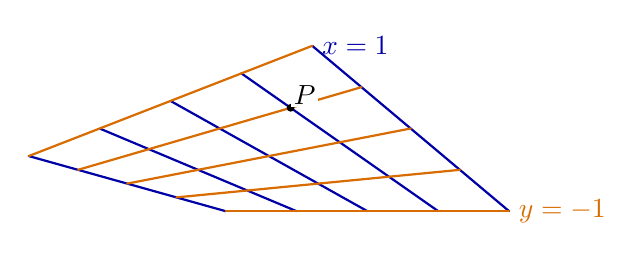
\begin{tikzpicture}[x={(1.8cm,0.35cm)},y={(-1.25cm,0.7cm)},z={(0cm,0.35cm)},line cap=round]
	\foreach \s in {-1,-0.5,0,0.5,1}{
		\draw[blue!65!black,thick] (\s,-1,{-\s}) -- (\s,1,\s);
	}
	\foreach \t in {-1,-0.5,0,0.5,1}{
		\draw[orange!85!black,thick] (-1,\t,{-\t}) -- (1,\t,\t);
	}
	\fill[black] (0.5,0.5,0.25) circle (1.4pt);
	\node[above right,fill=white,inner sep=1pt] at (0.5,0.5,0.25) {\(P\)};
	\node[blue!65!black,right] at (1,1,1) {\(x=1\)};
	\node[orange!85!black,right] at (1,-1,-1) {\(y=-1\)};
\end{tikzpicture}

	\caption[双曲抛物面的两个直纹族]{双曲抛物面 \(z=xy\) 的两个直纹族。蓝线固定 \(x\)，橙线固定 \(y\)，标出的点为 \(P=(1/2,1/2,1/4)\)。图中只画 \(-1\le x,y\le1\) 的部分，空间位置采用平行投影示意。两族线在曲面上相交，同族线互不相交。}
	\label{g1:fig:quadric-rulings}
\end{figure}

无中心标准形\eqref{g1:eq:affine-parabolic-quadric}可直接解出 \(z_1\)，因此总有实点，且是其他 \(n-1\) 个变量的图像；未出现的变量给出柱面的自由方向。有中心标准形中的自由变量也给出这种方向。例如 \(x^2+y^2=1\) 在 \(\mathbb R^3\) 中是一张圆柱面，虽然它的二次项矩阵有核，但其每一个实点附近都保持通常的圆柱形状。“矩阵有核”不能自动理解为实点集到处出现尖点或交叉。

\begin{example}[参数变化要看哪一项]
	\label{g1:exm:affine-quadric-degeneration}
	族 \(x^2+y^2=t\) 的二次项矩阵始终为 \(I_2\)，但当 \(t>0\)、\(t=0\)、\(t<0\) 时，实点集分别为圆、一个点、空集。改变的量是中心值 \(-t\)。另一族
	\[
		x^2+y^2-tz^2=1
	\]
	在 \(t<0\) 时为椭球面，\(t=0\) 时为圆柱面，\(t>0\) 时为单叶双曲面；后一名称对应截面圆半径 \(\sqrt{1+tz^2}\)，它对每个实数 \(z\) 都存在。这次发生变化的是二次项的秩与惯性。\cref{g1:prop:rank-inertia-continuity}说明，在连续实对称矩阵族中，秩固定时惯性局部不变；本例正是在 \(t=0\) 丢掉一个非零特征值，才从一个惯性类型走到另一个类型。
\end{example}

为了把二次项、线性项和常数项放进同一个对称矩阵，下一节引入一个齐次坐标。这会使上述两种看似不同的退化都能用一个齐次二次型描述，也会说明椭圆、抛物线和双曲线为何可能属于同一个射影类型。

% !TeX root = ../../Book1.tex
% 纲要标题：### 2.3 射影二次曲面与秩
% 纲要位置：几何学计划纲要.md，第 171 行。
% 正文状态：初稿；尚未正式审核。

% 纲要内容开始
% 
% * 齐次化及无穷远截面
% * 基域、秩和射影等价
% * 极大线性子空间及直纹族
% * 复化与实形式的不同分类信息
% 
% 纲要内容结束

\section{射影二次曲面与秩}
\label{g1:sec:0203}

仿射二次方程的三类系数在平移时互相混合，因此上一节的分类要分别讨论有无中心。齐次坐标提供了另一种看法：用新增坐标补齐次数，把所有项放进同一个二次型。这样可以直接使用合同分类，但代价是我们不再固定哪一个超平面被称作无穷远。椭圆、抛物线和双曲线的区别，恰好会在这个选择中重新出现。

\subsection{齐次化及无穷远截面}
\label{g1:subsec:0203:01}

设 \(F(x)=x^{\mathsf T}Ax+2b^{\mathsf T}x+c\) 是 \(K^n\) 上次数恰为二的多项式，其中 \(K=\mathbb R\) 或 \(\mathbb C\)，\(A\) 对称且非零。新增坐标 \(X_0\)，把原来的坐标写为 \(X=(X_1,\ldots,X_n)^{\mathsf T}\)，定义它的\term[qicihua]{齐次化}[homogenization]为
\begin{equation}
	\label{g1:eq:quadric-homogenization}
	\begin{aligned}
		F^{\mathrm h}(X_0,X)
		&=X^{\mathsf T}AX+2X_0b^{\mathsf T}X+cX_0^2\\
		&=\begin{pmatrix}X_0&X^{\mathsf T}\end{pmatrix}
		M\begin{pmatrix}X_0\\X\end{pmatrix},\\
		M&=\begin{pmatrix}c&b^{\mathsf T}\\b&A\end{pmatrix}.
	\end{aligned}
\end{equation}
它的每一项总次数都是二，所以向量整体乘以 \(t\ne0\) 时，函数值乘以 \(t^2\)；零值条件因此能在射影空间上定义。

\begin{definition}[射影二次曲面]
	\label{g1:def:projective-quadric}
	设 \(V\) 是有限维 \(K\) 向量空间，\(K=\mathbb R\) 或 \(\mathbb C\)，\(q\) 是 \(V\) 上非零二次型。由齐次方程 \(q=0\) 定义的\term[sheyingerciqumian]{射影二次曲面}[projective quadric]记为
	\[
		Q(q)=\{\,[v]\in\mathbb P(V):q(v)=0\,\}.
	\]
	讨论方程等价时，保留 \(q\) 到整体非零倍数的信息。其秩是对应对称矩阵的秩；矩阵可逆时称该二次曲面方程非退化，否则称其退化。
\end{definition}

在标准仿射图 \(X_0\ne0\) 中，用 \(x_i=X_i/X_0\)，有
\[
	F^{\mathrm h}(X_0,X)=X_0^2F(X/X_0).
\]
因此这个图中的零点恰好是原来的 \(F=0\)。在无穷远超平面 \(X_0=0\) 上，剩下的方程则是 \(X^{\mathsf T}AX=0\)。它记录二次项的零值方向，称为相对于这个仿射图的\term[wuqiongyuanjiemian]{无穷远截面}[section at infinity]。若把次数小于二的多项式也机械地补到二次，就可能多出整个无穷远超平面，例如线性方程 \(x_1=0\) 被写成 \(X_0X_1=0\)；这正是这里要求原方程次数恰为二的原因。

\begin{example}[三种实二次曲线的无穷远点]
	\label{g1:exm:conics-at-infinity}
	仿射平面中的三个方程齐次化后成为
	\[
		\begin{array}{c|c|c}
			\text{仿射方程}&\text{齐次方程}&\text{实无穷远点}\\ \hline
			x_1^2+x_2^2=1&X_1^2+X_2^2-X_0^2=0&\text{无}\\
			x_1^2-x_2^2=1&X_1^2-X_2^2-X_0^2=0&[0:1:1],\ [0:1:-1]\\
			x_1^2=x_2&X_1^2-X_0X_2=0&[0:0:1]
		\end{array}
	\]
	最后一行在无穷远超平面上的限制为平方 \(X_1^2\)，因此只给出一个实无穷远点。中间一行有两个不同的零值方向；第一行的正定二次项没有非零实零值方向。这里说的无穷远，始终相对于已经选定的 \(X_0=0\)。
\end{example}

在实数域上，还应区分齐次化与通常拓扑中的闭包。例如 \(x_1^2+1=0\) 在 \(\mathbb R^2\) 中没有实点，而齐次方程 \(X_1^2+X_0^2=0\) 在 \(\mathbb P^2(\mathbb R)\) 中有点 \([0:0:1]\)。所以齐次化的实零点集不必等于原实零点集的拓扑闭包。本节依据的是多项式和齐次坐标的计算，不把实点的逼近性质暗中放进“补入无穷远点”的说法中。

\ProseParagraphBreak

仿射坐标变换 \(x=Cy+a\) 在齐次坐标中对应可逆矩阵
\[
	T=\begin{pmatrix}1&0\\a&C\end{pmatrix}.
\]
它把 \((Y_0,Y)\) 送到 \((Y_0,aY_0+CY)\)，所以保持 \(X_0=0\)，并使 \(M\) 变为 \(T^{\mathsf T}MT\)。若允许任意可逆的 \((n+1)\) 阶矩阵，就不必再保持这个超平面，得到范围更大的射影等价关系。

\begin{proposition}[齐次化的秩]
	\label{g1:prop:homogenized-rank}
	设 \(F\) 是 \(\mathbb R^n\) 上次数恰为二的实多项式，二次项矩阵 \(A\) 的惯性为 \((p,q,r)\)，秩为 \(k=p+q\)。记齐次化矩阵为 \(M\)。
	\begin{enumerate}
		\item 若 \(F\) 有中心，中心值为 \(\kappa\)，则 \(M\) 合同于 \(\operatorname{diag}(\kappa,A)\)，其秩为 \(k\) 或 \(k+1\)，分别对应 \(\kappa=0\) 或 \(\kappa\ne0\)。
		\item 若 \(F\) 没有中心，则 \(\operatorname{rank}M=k+2\)，惯性为 \((p+1,q+1,r-1)\)。
	\end{enumerate}
\end{proposition}

\begin{proof}
	有中心时，把该中心移到原点，式\eqref{g1:eq:quadratic-translation}给出 \(F=y^{\mathsf T}Ay+\kappa\)，其齐次化矩阵正是 \(\operatorname{diag}(\kappa,A)\)。

	无中心时，\cref{g1:thm:euclidean-quadric-normal}给出 \(F=\sum_{i=1}^k\lambda_i y_i^2+2\beta z_1\)，其中 \(\beta>0\)。齐次化后，\(z_1\) 与新增坐标 \(Y_0\) 组成矩阵块
	\[
		\begin{pmatrix}0&\beta\\\beta&0\end{pmatrix},
	\]
	它在方向 \((1,1)\)、\((1,-1)\) 上分别有特征值 \(\beta\)、\(-\beta\)。所以它贡献一个正方向、一个负方向，原核中的其余 \(r-1\) 个方向仍为零。由此同时得到秩与惯性公式。
\end{proof}

这说明抛物线的二次项虽有核，齐次化的二次型却可以非退化；也说明一个有中心方程可能因中心值变成零而使齐次化的秩下降。对上一节的族 \(x^2+y^2=t\)，齐次化矩阵为 \(\operatorname{diag}(-t,1,1)\)，正好在 \(t=0\) 退化。

\subsection{基域、秩和射影等价}
\label{g1:subsec:0203:02}

对于 \(K=\mathbb R\) 或 \(\mathbb C\)，二次型 \(q\) 都对应唯一的对称双线性型
\[
	B(u,v)=\frac{q(u+v)-q(u)-q(v)}2.
\]
这与\cref{g1:def:symmetric-form}的实数情形相同。复数情形仍然对两个变量分别线性，矩阵公式是 \(u^{\mathsf T}Av\)，不含复共轭；它并不是用来测长度的复内积。根基仍定义为与所有向量配对均为零的向量组成的子空间。

\ProseParagraphBreak

在实数域上，惯性定理已经证明正负号无法通过实可逆换基消去；在复数域上，\(i^2=-1\) 却使 \(-x^2=(ix)^2\)。因此复数域上的分类应当更粗。为避免把实自伴谱定理误用到复对称矩阵上，我们直接给出所需的复数证明。

\begin{lemma}[复对称型的合同标准形]
	\label{g1:lem:complex-symmetric-normal}
	设 \(V\) 是 \(N\) 维复向量空间，\(B\) 是其上的对称双线性型，秩为 \(s\)。存在一组复基，使其矩阵为 \(\operatorname{diag}(I_s,0_{N-s})\)。两个同维复对称双线性型合同，当且仅当它们的秩相同。
\end{lemma}

\begin{proof}
	若 \(B=0\)，任意基都满足结论。若 \(B\ne0\)，则存在 \(v\) 使 \(B(v,v)\ne0\)：否则由极化公式，所有 \(B(u,v)\) 都为零。非零复数都有平方根，所以缩放 \(v\) 可得到 \(e\) 满足 \(B(e,e)=1\)。对任意 \(w\in V\)，分解
	\[
		w=B(w,e)e+\bigl(w-B(w,e)e\bigr)
	\]
	的第二项与 \(e\) 正交。并且 \(\mathbb Ce\cap e^\perp=0\)，因为 \(B(te,e)=t\)。这里 \(e^\perp\) 表示关于 \(B\) 的正交空间，故 \(V=\mathbb Ce\oplus e^\perp\)，在这个分解下矩阵为一个 \(1\) 与较低维对称型的直和。

	继续对后者归纳，直到剩下零型，就得到对角元只含 \(1\) 与 \(0\) 的矩阵。乘以可逆矩阵不改变秩，所以其中 \(1\) 的个数必为 \(s\)。这既给出数目唯一性，也说明秩相同的两个型都合同于同一个标准矩阵；反向蕴含由秩在合同变换下不变得到。
\end{proof}

\begin{theorem}[实、复射影二次方程的分类]
	\label{g1:thm:projective-quadric-classification}
	设 \(K=\mathbb R\) 或 \(\mathbb C\)，\(q,q'\) 是 \(N\) 维 \(K\) 向量空间上的非零二次型。称其射影方程等价，是指存在 \(T\in\operatorname{GL}(N,K)\) 及 \(\mu\in K\setminus\{0\}\)，使
	\[
		q'(v)=\mu q(Tv)\qquad(v\in K^N).
	\]
	在复数域上，等价的充要条件是二者秩相同。在实数域上，若惯性分别为 \((p,q_-,r)\) 与 \((p',q'_-,r')\)，等价的充要条件是
	\[
		r=r',\qquad \{p,q_-\}=\{p',q'_-\},
	\]
	其中花括号表示允许交换两个惯性指数的无序二元组。
\end{theorem}

\begin{proof}
	矩阵变化为 \(A' =\mu T^{\mathsf T}AT\)，故任何基域上秩都保持不变。复数情形由\cref{g1:lem:complex-symmetric-normal}，相同秩已足以给出合同，甚至不必再乘一个标量。

	实数情形由\cref{g1:thm:inertia}，合同保持 \((p,q_-,r)\)。乘以正数不改变这三个数；乘以负数则交换正、负惯性指数，保持根基维数。故所列条件必要。若条件成立，两组惯性相同，或把其中一个型乘以 \(-1\) 后相同；再用惯性定理的标准形便得到所需合同，故条件也充分。
\end{proof}

这里用 \(q_-\) 表示负惯性指数，是为了与二次型 \(q\) 区别；下面没有这种冲突时仍写惯性为 \((p,q,r)\)。定理分类的是方程及其基域，不只是肉眼所见的实点形状。例如在 \(\mathbb P^2(\mathbb R)\) 中，方程 \(X_0^2=0\) 与 \(X_0^2+X_1^2=0\) 的实零点集分别是一条直线与一个点；它们的秩分别为 \(1,2\)。即使两个方程的实零点集偶然相同，也不能因此认定它们按上述定义等价。

\begin{example}[椭圆、双曲线和抛物线的射影类型]
	\label{g1:exm:one-projective-conic-type}
	\cref{g1:exm:conics-at-infinity}中的三个齐次型都具有秩 \(3\)，正、负惯性指数的无序二元组均为 \(\{2,1\}\)，所以它们的实射影方程等价。第三个式子中，\(-X_0X_2\) 在 \(X_0+X_2\) 与 \(X_0-X_2\) 两个方向上给出相反符号，再加上 \(X_1^2\) 就能直接核对惯性。它们作为仿射曲线仍然不同，因为给出等价的射影变换不必保持已选的无穷远直线。区分“曲线”与“曲线加上一条指定的无穷远直线”，就能同时理解这两个结论。
\end{example}

\subsection{极大线性子空间及直纹族}
\label{g1:subsec:0203:03}

一个射影点 \([v]\) 在 \(Q(q)\) 上，只要求 \(q(v)=0\)。若希望整条射影直线、甚至更高维的射影子空间都在曲面上，就必须要求它的全部向量都满足这个条件。由\cref{g1:prop:projective-dimension}，\(k\) 维射影子空间来自 \(k+1\) 维向量子空间；因此以下问题可以完全化成双线性型问题。

\begin{definition}[全迷向子空间]
	\label{g1:def:totally-isotropic}
	设 \(V\) 是实或复向量空间，\(B\) 是对称双线性型，\(q(v)=B(v,v)\)。子空间 \(U\subseteq V\) 若满足 \(q|_U=0\)，称为\term[quanmixiangzikongjian]{全迷向子空间}[totally isotropic subspace]。等价地，\(B(u,w)=0\) 对所有 \(u,w\in U\) 成立；等价性由极化公式得到。不能真包含于更大全迷向子空间中的 \(U\) 称为极大，而可能达到的最大维数还需证明。
\end{definition}

注意，全迷向条件要求子空间内任意两个向量之间的配对也为零。两个分别迷向的向量未必张成全迷向平面：对 \(x^2-y^2\)，\((1,1)\) 与 \((1,-1)\) 都迷向，但它们的和为 \((2,0)\)，二次型值为 \(4\)。

\begin{theorem}[二次曲面中的最大线性维数]
	\label{g1:thm:quadric-linear-dimension}
	设 \(V\) 是 \(N\) 维实或复向量空间，\(q\ne0\) 是二次型，对应型为 \(B\)，根基维数为 \(r\)。
	\begin{enumerate}
		\item 若基域为实数，\(B\) 的惯性为 \((p,q_-,r)\)，则全迷向子空间的最大维数为
		\[
			r+\min(p,q_-).
		\]
		\item 若基域为复数，\(B\) 的秩为 \(s=N-r\)，则该最大维数为
		\[
			r+\lfloor s/2\rfloor.
		\]
	\end{enumerate}
	每个按包含关系极大的全迷向子空间都达到相应最大维数。若该数为 \(d>0\)，则 \(Q(q)\) 中最大射影线性子空间的维数为 \(d-1\)；若 \(d=0\)，则 \(Q(q)\) 没有基域内的点。
\end{theorem}

\begin{proof}
	先处理根基。由标准形可取直和 \(V=R\oplus W\)，其中 \(R=\operatorname{rad}B\)，\(B|_W\) 非退化。任意全迷向子空间 \(U\) 投影到 \(W\) 的像 \(\overline U\) 仍全迷向，而且
	\[
		\dim U=\dim(U\cap R)+\dim\overline U
		\le r+\dim\overline U.
	\]
	反过来，\(W\) 中的全迷向子空间与 \(R\) 直和仍全迷向。所以最大维数等于 \(r\) 加上非退化部分中的最大维数。

	在实非退化情形，标准形为 \(\lVert x\rVert^2-\lVert y\rVert^2\)，其中 \(x\in\mathbb R^p\)、\(y\in\mathbb R^{q_-}\)。对全迷向子空间，投影到任一组坐标都是单射：例如 \(x=0\) 时，零值条件给出 \(\lVert y\rVert^2=0\)，迫使 \(y=0\)。所以其维数同时不超过 \(p\) 与 \(q_-\)。取正、负标准基 \(e_i,f_j\)，向量
	\[
		e_1+f_1,\ldots,e_m+f_m,
		\qquad m=\min(p,q_-),
	\]
	彼此配对均为零，且线性无关，故上界可达到。

	在复非退化的 \(s\) 维空间中，若 \(U\) 全迷向，则 \(U\subseteq U^\perp\)。这里 \(\dim U^\perp=s-\dim U\)：非退化性使 \(w\mapsto B(w,-)\) 成为到对偶空间的同构，而任意 \(U\) 上的线性函数都可以先扩充一组基，再延拓到全空间；因此 \(w\mapsto B(w,-)|_U\) 满射到 \(U^*\)，其核就是 \(U^\perp\)。秩与零化度公式给出所需维数。于是 \(2\dim U\le s\)。在\cref{g1:lem:complex-symmetric-normal}的标准基中，
	\[
		e_1+ie_2,\ e_3+ie_4,\ldots,
		e_{2m-1}+ie_{2m},\qquad m=\lfloor s/2\rfloor,
	\]
	构成线性无关的全迷向向量组，故复数情形的上界也可达到。

	最后证明极大子空间不可能停在更小的维数。极大全迷向子空间必包含 \(R\)，否则加上根基中的一个新方向仍然全迷向；此时它等于 \(R\oplus(U\cap W)\)。于是只需在非退化部分中证明结论，仍把其中的全迷向子空间记为 \(U\)。若 \(u\in U\) 非零，非退化性给出 \(v\) 满足 \(B(u,v)=1\)。以
	\[
		v'=v-\frac{B(v,v)}2u
	\]
	替代 \(v\)，就有 \(B(v',v')=0\)、\(B(u,v')=1\)。平面 \(H=\operatorname{span}(u,v')\) 的配对矩阵为 \(\left(\begin{smallmatrix}0&1\\1&0\end{smallmatrix}\right)\)，因而非退化。任意 \(w\) 都可按
	\[
		w=B(w,v')u+B(w,u)v'
		+\bigl(w-B(w,v')u-B(w,u)v'\bigr)
	\]
	分成 \(H\) 与 \(H^\perp\) 两部分，且交集为零。\(H^\perp\) 上的限制仍非退化：若其中一个向量与整个 \(H^\perp\) 正交，它也与 \(H\) 正交，便与整个空间正交，故只能为零。若 \(w\in U\)，则 \(B(w,u)=0\)，所以 \(U=Ku\oplus(U\cap H^\perp)\)。

	重复这一步，若 \(\dim U=k\)，便剥离出 \(k\) 个这样的二维平面，余下非退化空间 \(W_0\) 与它们正交。在实数域中每剥离一次，正、负惯性指数各减一，所以若 \(k<\min(p,q_-)\)，\(W_0\) 仍有一正一负两个方向；它们可组成新的迷向向量。在复数域中，若 \(k<\lfloor s/2\rfloor\)，则 \(\dim W_0\ge2\)，也可由标准形的前两个方向组成 \(e_1+ie_2\)。这些新向量都与原 \(U\) 正交，使 \(U\) 真正扩大，违背极大性。这也覆盖 \(U=0\) 而上界为正的情形。

	最后，非零全迷向子空间 \(U\) 与曲面内的射影子空间 \(\mathbb P(U)\) 恰好对应，其维数减少一。若不存在非零全迷向子空间，连一个迷向向量都不存在，曲面便没有相应基域的射影点。
\end{proof}

定理中的两个维数计数揭示了实、复几何的差别。例如实球面齐次化后的型为 \(X_1^2+X_2^2+X_3^2-X_0^2\)，惯性为 \((3,1,0)\)。全迷向子空间最大只有一维，所以球面射影化后没有实射影直线。允许复坐标以后，同一个矩阵秩为 \(4\)，最大全迷向维数变为二，因而出现复射影直线。

\ProseParagraphBreak

对于惯性 \((2,2,0)\) 的实型，最大射影线性子空间就是直线。下面的模型不仅表明直线存在，而且把它们全部写出。这个表示也将在\secref{g1:sec:0206}中成为一个射影映射的例子。

\begin{proposition}[二次曲面的两个直纹族]
	\label{g1:prop:quadric-two-rulings}
	设 \(K=\mathbb R\) 或 \(\mathbb C\)，在 \(\mathbb P^3(K)\) 中考虑
	\[
		Q:\ X_0X_3-X_1X_2=0.
	\]
	每个点唯一写为
	\begin{equation}
		\label{g1:eq:quadric-rank-one-param}
		[X_0:X_1:X_2:X_3]
		=[su:sv:tu:tv],
		\qquad [s:t],[u:v]\in\mathbb P^1(K).
	\end{equation}
	固定 \([s:t]\) 而让 \([u:v]\) 变化，或固定 \([u:v]\) 而让 \([s:t]\) 变化，各得到一个直纹族。这两族包含 \(Q\) 上的全部射影直线；同族不同直线互不相交，异族任意两条直线恰交于一点。过 \(Q\) 上的每一点恰有两条直线，每族各一条。
\end{proposition}

\begin{proof}
	把四个坐标排成矩阵
	\[
		Z=\begin{pmatrix}X_0&X_1\\X_2&X_3\end{pmatrix}.
	\]
	方程是 \(\det Z=0\)，而射影坐标要求 \(Z\ne0\)，所以 \(Z\) 的秩恰为一。选一个非零列，其他列都是它的倍数，便可写成 \(Z=a b^{\mathsf T}\)，其中非零列向量 \(a=(s,t)^{\mathsf T}\)、\(b=(u,v)^{\mathsf T}\)。它的列空间决定 \([a]\)，行空间决定 \([b]\)，故这两个射影点都唯一。分别改变 \(a,b\) 的代表，只把 \(Z\) 整体乘以非零数，所以式\eqref{g1:eq:quadric-rank-one-param}良定义。

	固定非零 \(a\) 后，映射 \(b\mapsto ab^{\mathsf T}\) 线性且单射，因此其像是二维向量子空间，射影化后正是一条直线；固定 \(b\) 同理。分解的唯一性说明同族不同直线没有公共点，而分别固定 \([a]\)、\([b]\) 的异族两条线只在 \([ab^{\mathsf T}]\) 相交。

	还须排除第三种直线。设 \(L\subseteq Q\) 为任意射影直线，取它对应二维向量空间的一组基 \(ab^{\mathsf T}\)、\(cd^{\mathsf T}\)。对所有 \(\tau\in K\)，矩阵 \(ab^{\mathsf T}+\tau cd^{\mathsf T}\) 的行列式为零。按两列展开，得到
	\[
		\det\bigl(ab^{\mathsf T}+\tau cd^{\mathsf T}\bigr)
		=\tau\det(a,c)\det(b,d).
	\]
	取 \(\tau=1\)，可知 \(a,c\) 成比例或 \(b,d\) 成比例；二者不能同时成比例，否则两基向量相关。在第一种情形，整条 \(L\) 属于固定 \([a]\) 的族；在第二种情形，属于固定 \([b]\) 的族。全部断言随之成立。
\end{proof}

在图 \(X_0\ne0\) 中令 \(x=X_1/X_0\)、\(y=X_2/X_0\)、\(z=X_3/X_0\)，方程成为 \(z=xy\)，两个直纹族正是上一节画出的固定 \(x\) 与固定 \(y\) 的直线族。不过射影曲面还包含无穷远处的两条线：把 \(X_0=0\) 代入，得到 \(X_1X_2=0\)，即 \(X_0=X_1=0\) 与 \(X_0=X_2=0\)。它们也各属于一个直纹族，交于 \([0:0:0:1]\)，因此射影描述补全了仿射图没有显示的直线。

\subsection{复化与实形式的不同分类信息}
\label{g1:subsec:0203:04}

一个实二次方程可以保持系数不变而允许复数坐标，这称为把方程\term[fuhua]{复化}[complexification]。矩阵的秩不变，因为某阶子式是否非零不因把实数看成复数而改变；惯性的正负号却不再是复换基的不变量。乘以 \(i\) 就能把一个正平方改成负平方，因而所有相同秩的复二次型归入同一类。

\ProseParagraphBreak

为说明丢掉了哪些信息，\cref{g1:tab:real-quadric-forms}比较 \(\mathbb P^3(\mathbb R)\) 中的三种满秩方程。它们的复化都具有秩 \(4\)，所以由\cref{g1:thm:projective-quadric-classification}彼此复射影等价。

\begin{table}[htbp]
	\centering
	\caption{同一个复二次曲面类型的不同实形式}
	\label{g1:tab:real-quadric-forms}
	\begin{tabularx}{\linewidth}{@{}l c X@{}}
		\toprule
		实齐次方程 & 惯性 & 实几何 \\
		\midrule
		\(X_0^2+X_1^2+X_2^2+X_3^2=0\) & \((4,0,0)\) & 没有实点 \\
		\(X_1^2+X_2^2+X_3^2-X_0^2=0\) & \((3,1,0)\) & 有实点，没有实直线 \\
		\(X_0X_3-X_1X_2=0\) & \((2,2,0)\) & 有两个实直纹族 \\
		\bottomrule
	\end{tabularx}
\end{table}

第一行中，正定性排除了非零实零值向量；第二行在 \(X_0=1\) 中就是单位球面，维数定理已经说明它不含实直线；第三行则由两个符号相反的乘积各贡献一个正、一个负方向，且直纹由\cref{g1:prop:quadric-two-rulings}完全描述。这三种实方程可称为该复射影类型的不同\term[shixingshi]{实形式}[real forms]：它们的复化等价，但实数域上的方程并不等价。这里的名称只用于这项具体比较，不预设一般实形式理论。

\ProseParagraphBreak

由实到复并非简单地给图上每一点再加一个虚部。实点的存在、实直线的存在和实惯性都可能在复化后不再可辨；保存下来的秩则仍然控制根基维数及最大复线性子空间维数。后面讨论极性时，非退化性还会决定一个点能否唯一对应一个超平面。因此，在说“二次曲面由秩分类”以前，必须先说明基域；在说“这个曲面有直纹”以前，也必须说明这些直线在哪个基域上定义。

% !TeX root = ../../Book1.tex
% 纲要标题：### 2.4 射影对偶与极性
% 纲要位置：几何学计划纲要.md，第 178 行。
% 正文状态：初稿；尚未正式审核。

% 纲要内容开始
% 
% * 超平面参数空间与双重对偶
% * 非退化配对产生的极点、极超平面
% * 切空间、切超平面与对偶二次曲面
% * 退化配对中极性的失效
% 
% 纲要内容结束

\section{射影对偶与极性}
\label{g1:sec:0204}

平面上一点写成齐次坐标 \([x_0:x_1:x_2]\)，一条直线也由一组非全零系数 \([a_0:a_1:a_2]\) 决定，其方程是 \(a_0x_0+a_1x_1+a_2x_2=0\)。点的坐标与直线的系数虽然形式相似，却属于不同的向量空间。先保留这个区别，再利用二次型建立二者的对应，就能说明为什么一条共线定理会产生另一条共点定理，也能把二次曲面的切超平面组织成新的二次曲面。

\subsection{超平面参数空间与双重对偶}
\label{g1:subsec:0204:01}

设 \(V\) 是 \(K=\mathbb R\) 或 \(\mathbb C\) 上的 \(n+1\) 维向量空间，\(n\ge1\)。回顾对偶空间 \(V^*\) 的元素是线性函数 \(\alpha:V\rightarrow K\)。每个非零 \(\alpha\) 给出射影超平面 \(H_\alpha=\mathbb P(\ker\alpha)\)。两个非零函数给出同一超平面，当且仅当相差非零倍数：若核相同，取 \(v\) 使 \(\alpha(v)=1\)，分解 \(x=\alpha(x)v+(x-\alpha(x)v)\)，即得 \(\beta(x)=\beta(v)\alpha(x)\)。反之，乘非零常数不改变核。每个余维一子空间都是某个非零函数的核，因为可以取它的一组基，补上一个向量，并令线性函数在前者上为零、在补上的向量上为 \(1\)。

\begin{definition}[射影对偶空间]\label{g1:def:projective-dual}
	对于 \(K=\mathbb R\) 或 \(\mathbb C\) 上有限维向量空间 \(V\)，称 \(\mathbb P(V^*)\) 为 \(\mathbb P(V)\) 的\term[sheyingduioukongjian]{射影对偶空间}[dual projective space]。其中一点 \([\alpha]\) 参数化原空间的超平面 \(H_\alpha\)。点 \([v]\) 与超平面 \([\alpha]\) 的关联条件是 \(\alpha(v)=0\)。
\end{definition}

这个条件对 \(v,\alpha\) 的非零倍数都不变。在选定的基及其对偶基中，它是 \(\sum_i a_ix_i=0\)；但把点坐标列直接当成超平面系数列，需要额外选择，不能仅凭两列有同样长度就认作自然对应。真正不需要选基的是到双重对偶的求值映射
\[
	\iota:V\longrightarrow V^{**},\qquad
	\iota(v)(\alpha)=\alpha(v).
\]
若 \(v\ne0\)，把 \(v\) 扩充成基便可构造 \(\alpha(v)=1\) 的函数，所以 \(\iota\) 单射。取一组基可知 \(\dim V^*=\dim V\)，再用一次得到 \(\dim V^{**}=\dim V\)，故 \(\iota\) 是同构。因此双重射影对偶自然回到原空间。

\begin{proposition}[零化子与关联反转]\label{g1:prop:annihilator-duality}
	设 \(V\) 是 \(K=\mathbb R\) 或 \(\mathbb C\) 上的有限维向量空间，\(U,W\subseteq V\) 为子空间。定义 \(U\) 的\term[linghuazi]{零化子}[annihilator]
	\[
		U^\circ\coloneqq\{\,\alpha\in V^*: \alpha(u)=0\text{ 对一切 }u\in U\,\}.
	\]
	经由求值同构把 \(V^{**}\) 认作 \(V\)，有
	\[
		\begin{gathered}
			\dim U^\circ=\dim V-\dim U,\qquad (U^\circ)^\circ=U,\\
			(U+W)^\circ=U^\circ\cap W^\circ,\qquad
			(U\cap W)^\circ=U^\circ+W^\circ.
		\end{gathered}
	\]
	因此取零化子反转包含关系，也将射影子空间的张成与相交互换。
\end{proposition}
\begin{proof}
	把 \(U\) 的基 \(u_1,\ldots,u_k\) 补成 \(V\) 的基 \(u_1,\ldots,u_m\)。其对偶基中最后 \(m-k\) 个函数构成 \(U^\circ\) 的基，得到维数公式。每个 \(u\in U\) 被 \(U^\circ\) 中的所有函数零化，故 \(U\subseteq(U^\circ)^\circ\)；两边维数均为 \(k\)，于是相等。

	一个函数在 \(U+W\) 上为零，当且仅当它同时在 \(U,W\) 上为零，得到第一条运算公式。再在 \(V^*\) 中对 \(U^\circ,W^\circ\) 使用这条公式，得 \((U^\circ+W^\circ)^\circ=U\cap W\)；取第二次零化子便得到另一条。最后，\(U\subseteq W\) 直接推出 \(W^\circ\subseteq U^\circ\)。
\end{proof}
\symidx{\(U^\circ\)：子空间的零化子}

若 \(\dim\mathbb P(V)=n\)，则一个 \(k\) 维射影子空间对应一个 \(n-k-1\) 维对偶子空间。采用 \(\mathbb P(0)=\varnothing\)、维数 \(-1\) 的约定时，整个空间与空集也互相对应。在射影平面中，点与直线互换；两点的连线与两条对偶直线的交点互换。三个点共线，等价于它们的代表向量张成空间维数至多为 \(2\)，也等价于三个对偶直线具有公共点。这些结论来自零化子公式，不需要图形的位置猜测。

\subsection{非退化配对产生的极点、极超平面}
\label{g1:subsec:0204:02}

射影对偶把原空间与另一个空间联系起来。若还想在原空间内部给每一点指定一个超平面，就需要一个从 \(V\) 到 \(V^*\) 的同构。对称双线性型恰好提供这样的映射，而且它的对称性将变成几何上的互反关系。

\begin{definition}[二次型的极性]\label{g1:def:quadric-polarity}
	设 \(V\) 是 \(K=\mathbb R\) 或 \(\mathbb C\) 上维数至少为 \(2\) 的向量空间， \(B\) 是非退化对称双线性型。记
	\[
		b:V\longrightarrow V^*,\quad b(v)=B(v,-),\qquad
		U^{\perp_B}=\{\,w\in V:B(u,w)=0\text{ 对一切 }u\in U\,\}.
	\]
	点 \(p=[v]\) 的\term[jichaopingmian]{极超平面}[polar hyperplane]是 \(p^{\perp_B}=\mathbb P((Kv)^{\perp_B})\)；超平面 \(H_\alpha\) 的\term[jidian]{极点}[pole]是 \([b^{-1}\alpha]\)。这一反转关联的对应称为由 \(B\) 给出的\term[jixing]{极性}[polarity]。在射影平面中，极超平面通常称为\term[jixian]{极线}[polar line]。
\end{definition}

非退化的含义仍是 \(B(v,w)=0\) 对所有 \(w\) 成立时必有 \(v=0\)，与\cref{g1:def:symmetric-form}的实情形相同。它保证 \(b\) 单射；有限维且两端同维又保证 \(b\) 满射，所以上述逆映射确实存在。把 \(B\) 乘以非零常数不改变极性。这里只使用双线性型；在复数域上不作复共轭，不能把它换成带复共轭的内积而仍沿用相同公式。

\begin{proposition}[极性的互反性]\label{g1:prop:polarity}
	设 \(V\) 是 \(K=\mathbb R\) 或 \(\mathbb C\) 上 \(n+1\) 维向量空间，\(n\ge1\)， \(B\) 为非退化对称双线性型。对每个子空间 \(U\subseteq V\)，有
	\[
		\dim U^{\perp_B}=n+1-\dim U,\qquad
		(U^{\perp_B})^{\perp_B}=U.
	\]
	对点 \(p=[v]\)、\(q=[w]\)，有
	\[
		p\in q^{\perp_B}\quad\Longleftrightarrow\quad q\in p^{\perp_B}.
	\]
	点 \(p\) 落在自己的极超平面上，当且仅当 \(B(v,v)=0\)。
\end{proposition}
\begin{proof}
	对称性给出 \(U^{\perp_B}=b^{-1}(U^\circ)\)，故维数公式由\cref{g1:prop:annihilator-duality}得到。又有 \(U\subseteq(U^{\perp_B})^{\perp_B}\)，因为 \(B(u,w)=B(w,u)\)；两边维数相同，故相等。点的互反性正是 \(B(w,v)=0\) 与 \(B(v,w)=0\) 的等价，最后令 \(w=v\) 即得自关联条件。
\end{proof}

因此二次曲面 \(Q=\{\,[v]:B(v,v)=0\,\}\) 可以从极性中恢复为所有自关联点。反过来，给定二次方程及其对称配对便得到极性。这里仍应记住前两节对方程与点集的区别：例如正定实型的射影零点集为空，但它给出的极性存在，并且绝不由“空集”这一个集合唯一决定。

\begin{example}[圆的极线]\label{g1:exm:circle-polar}
	在 \(\mathbb P^2(\mathbb R)\) 中考虑 \(X^2+Y^2-Z^2=0\)。点 \([a:b:c]\) 的极线是 \(aX+bY-cZ=0\)。在仿射图 \(Z=1\) 中，点 \((2,0)\) 的极线是 \(x=1/2\)，圆心 \([0:0:1]\) 的极线则是无穷远直线 \(Z=0\)。无穷远点 \([1:0:0]\) 的极线为直径所在的直线 \(X=0\)。这些计算说明极线不要求通过原来的点；只有圆上的点才有这一性质。
\end{example}

\subsection{切空间、切超平面与对偶二次曲面}
\label{g1:subsec:0204:03}

为什么极线与圆锥曲线的切线有关？沿着一条过曲面上点的直线代入二次方程，常数项已经为零，一次项描述离开曲面的第一阶变化；令一次项为零，恰好得到极超平面的方程。下面把这个观察写成不依赖图像的局部计算。

\begin{proposition}[二次曲面的线性化]\label{g1:prop:quadric-tangent}
	设 \(K=\mathbb R\) 或 \(\mathbb C\)，\(\dim V=n+1\)、\(n\ge2\)， \(B\) 为对称双线性型，\(Q\subseteq\mathbb P(V)\) 由 \(q(x)=B(x,x)=0\) 定义。设 \(p=[v]\in Q\)，且 \(B(v,-)\ne0\)。则 \(Q\) 在 \(p\) 处的一阶方程给出唯一的射影超平面
	\[
		\mathrm{T}_pQ=\mathbb P\{\,w\in V:B(v,w)=0\,\}.
	\]
	选取 \(\alpha\in V^*\) 满足 \(\alpha(v)=1\)，在仿射图 \(\alpha=1\) 内，切向量组成的空间是
	\[
		\{\,u\in\ker\alpha:B(v,u)=0\,\},
	\]
	其 \(K\)-维数为 \(n-1\)，并通过商映射同构于 \(\ker B(v,-)/Kv\)。
\end{proposition}
\begin{proof}
	仿射图中以 \(v\) 为基点，每一点写成 \(v+u\)，其中 \(u\in\ker\alpha\)。代入得
	\[
		q(v+u)=2B(v,u)+q(u),
	\]
	因为 \(q(v)=0\)。因此一阶线性部分为 \(u\mapsto2B(v,u)\)。它在 \(\ker\alpha\) 上非零：否则 \(B(v,-)\) 是 \(\alpha\) 的倍数，把 \(v\) 代入得倍数为 \(B(v,v)=0\)，与假设矛盾。所以其核在 \(n\) 维方向空间 \(\ker\alpha\) 中有余维一。

	一阶仿射平面由 \(v+u\)、\(\alpha(u)=B(v,u)=0\) 组成。其射影张成空间为 \(\mathbb P(\ker B(v,-))\)：对任何 \(w\in\ker B(v,-)\)，分解 \(w=\alpha(w)v+(w-\alpha(w)v)\)，后项同时属于两个核。同一分解也说明商映射将切向量空间一一对应到 \(\ker B(v,-)/Kv\)。换另一个仿射图时仍得到同一个齐次超平面；把 \(v\) 换成非零倍数也不改变其核。
\end{proof}

这里将方程的一阶部分非零的点称为该二次方程的\term[guanghuadian]{光滑点}[smooth point]，将 \(\mathrm{T}_pQ\) 称为\term[qiechaopingmian]{切超平面}[tangent hyperplane]。上述仿射图中的方向空间是\term[qiekongjian]{切空间}[tangent space]的当前坐标描述；当 \(n=2\) 时，切超平面就是\term[qiexian]{切线}[tangent line]。我们在这里用多项式的一阶项定义这些对象，不需要预先调用隐函数定理。若一条过 \(p\) 的直线由 \(v,w\) 张成，则
\[
	q(v+tw)=2tB(v,w)+t^2q(w).
\]
它的方向落在切超平面中，恰好表示一次项消失；若二次项也消失，整条直线就在 \(Q\) 上。因此在含有直纹的二次曲面上，“切”不排除整条直线包含在曲面内。

\begin{theorem}[非退化二次曲面的对偶]\label{g1:thm:dual-quadric}
	设 \(K=\mathbb R\) 或 \(\mathbb C\)，\(n\ge2\)， \(A\) 为可逆的 \((n+1)\times(n+1)\) 对称矩阵， \(Q=\{\,[x]\in\mathbb P^n(K):x^{\mathsf T}Ax=0\,\}\)。以超平面系数 \([a]\) 为对偶坐标，所有 \(Q\) 的切超平面组成\term[duiouerciqumian]{对偶二次曲面}[dual quadric]
	\[
		Q^*=\{\,[a]\in\mathbb P((K^{n+1})^*):a^{\mathsf T}A^{-1}a=0\,\}.
	\]
	映射 \([x]\mapsto[Ax]\) 在 \(Q\) 与 \(Q^*\) 间给出双射；对 \(Q^*\) 再作同样的对偶构造，返回 \(Q\)。
\end{theorem}
\begin{proof}
	对 \([x]\in Q\)，可逆性保证 \(Ax\ne0\)，所以\cref{g1:prop:quadric-tangent}适用，其切超平面系数为 \(a=Ax\)。由对称性，
	\[
		a^{\mathsf T}A^{-1}a=x^{\mathsf T}Ax=0.
	\]
	反过来，若 \(a^{\mathsf T}A^{-1}a=0\)，令 \(x=A^{-1}a\)，则 \(x\ne0\)，且 \(x^{\mathsf T}Ax=0\)；在这个点的切超平面恰为 \([a]\)。两个映射互为逆，且将 \(A\) 换为 \(A^{-1}\) 再作一次便返回原方程。若实零点集为空，上述两个集合同时为空，这个集合等式和矩阵公式仍然成立。
\end{proof}

\begin{example}[切线的参数方程]\label{g1:exm:dual-conic}
	对圆锥曲线 \(XZ-Y^2=0\)，可取
	\[
		A=\begin{pmatrix}0&0&1/2\\0&-1&0\\1/2&0&0\end{pmatrix}.
	\]
	在点 \([s^2:st:t^2]\) 处的切线为 \(t^2X-2stY+s^2Z=0\)。所以切线系数 \([a:b:c]=[t^2:-2st:s^2]\) 满足 \(b^2-4ac=0\)。这也是由 \(a^{\mathsf T}A^{-1}a=0\) 得到的方程。一族切线之所以能成为对偶平面中的曲线，是因为每条线由一个系数点表示；两边的“点”分别参数化不同种类的几何对象。
\end{example}

\subsection{退化配对中极性的失效}
\label{g1:subsec:0204:04}

退化时不应只在非退化公式中删掉一个逆矩阵符号。若 \(R=\operatorname{rad}B\ne0\)，映射 \(b:v\mapsto B(v,-)\) 的核为 \(R\)，像为 \(R^\circ\)：像包含于 \(R^\circ\) 是对称性的结果，两者维数都等于 \(\dim V-\dim R\)。因此 \([v]\in\mathbb P(R)\) 对应零函数，根本没有极超平面；在其余点，\([v]\mapsto[B(v,-)]\) 仍有定义，但 \(v\) 与 \(v+r\) 给出相同函数，通常不再单射。得到的每个超平面还都包含 \(\mathbb P(R)\)，故也不能遍历全部超平面。

\begin{proposition}[退化型的双重正交补]\label{g1:prop:degenerate-polarity}
	设 \(V\) 是 \(K=\mathbb R\) 或 \(\mathbb C\) 上的有限维向量空间， \(B\) 为对称双线性型，\(R=\operatorname{rad}B\)。则对每个子空间 \(U\subseteq V\)，
	\[
		(U^{\perp_B})^{\perp_B}=U+R.
	\]
	在商空间 \(V/R\) 上，公式 \(\overline B(v+R,w+R)=B(v,w)\) 定义非退化对称双线性型。
\end{proposition}
\begin{proof}
	改变代表向量只会增加根基中的向量，所有新增配对项为零，所以 \(\overline B\) 良定义。若 \(\overline B(v+R,w+R)=0\) 对所有 \(w\) 成立，则 \(v\in R\)，证明非退化性。记商映射为 \(\pi:V\rightarrow V/R\)。由定义， \(U^{\perp_B}=\pi^{-1}((\pi U)^{\perp_{\overline B}})\)。在商空间使用\cref{g1:prop:polarity}的双重正交补结论，再取逆像，得到 \((U^{\perp_B})^{\perp_B}=\pi^{-1}(\pi U)=U+R\)。商空间维数为 \(0\) 或 \(1\) 时，所用向量空间公式仍由同一维数证明成立。
\end{proof}

\begin{example}[锥顶与重合的切平面]\label{g1:exm:singular-polarity}
	在 \(\mathbb P^3(\mathbb R)\) 中，令 \(q(X,Y,Z,W)=X^2+Y^2-Z^2\)。根基为 \(\mathbb R(0,0,0,1)\)，锥顶 \([0:0:0:1]\) 处一次项全为零，没有由一阶方程确定的切平面。对每个 \(w\in\mathbb R\)，点 \([1:0:1:w]\) 在二次曲面上，其切平面都为 \(X-Z=0\)。这些点沿一条母线变化，切平面却不变，展示了对偶映射丢失的自由度。
\end{example}

更极端地，在射影平面中，方程 \(X^2=0\) 的实点集和复点集都是直线 \(X=0\)，但作为这个二次方程，它在每个点的一阶部分都为零。若把它先改成一次方程 \(X=0\)，当然得到一条光滑直线；这已经更换了定义方程所保留的信息。所以本节对退化对象的线性化始终针对给定的二次方程，不能仅从裸点集判断其一阶结构。

% !TeX root = ../../Book1.tex
% 纲要标题：### 2.5 圆锥曲线上的构造与定理
% 纲要位置：几何学计划纲要.md，第 185 行。
% 正文状态：初稿；尚未正式审核。

% 纲要内容开始
% 
% * 由投影得到有理参数及其逆
% * 圆锥曲线上的交比
% * Pascal 定理的坐标证明
% * Brianchon 定理与对偶推导
% 
% 纲要内容结束

\section{圆锥曲线上的构造与定理}
\label{g1:sec:0205}

射影分类告诉我们哪些圆锥曲线可以通过换坐标互相变换，但还没有说明怎样在一条曲线上移动和构造点。一个可操作的办法是固定曲线上一点，让过它的直线转动，用直线与曲线的另一个交点作参数。这样，圆锥曲线上的计算转化为射影直线上的计算；交比因此有了新的适用对象，而六个点的关联关系也能压缩为含三个参数的多项式恒等式。

\subsection{由投影得到有理参数及其逆}
\label{g1:subsec:0205:01}

本节讨论 \(K=\mathbb R\) 或 \(\mathbb C\) 上的非退化圆锥曲线，即射影平面中由可逆对称矩阵给出的二次方程。实数域上还须要求存在实点；例如 \(X^2+Y^2+Z^2=0\) 没有实射影点，不能从 \(\mathbb P^1(\mathbb R)\) 参数化一个空集。由\cref{g1:thm:projective-quadric-classification}，复数域上的非退化三元型都等价于 \(X^2+Y^2+Z^2\)，它含有点 \([1:\mathrm i:0]\)，所以在复数域上非空条件自动满足。下面仍把一个曲线点作为构造的输入，从它直接找出参数坐标。

\begin{proposition}[圆锥曲线的参数化]\label{g1:prop:conic-parametrization}
	设 \(K=\mathbb R\) 或 \(\mathbb C\)，\(C\subseteq\mathbb P^2(K)\) 是非退化圆锥曲线，且有一个 \(K\)-点。则存在射影坐标使 \(C\) 的方程为 \(XZ-Y^2=0\)。在这些坐标中，映射
	\begin{equation}\label{g1:eq:conic-parametrization}
		\nu:\mathbb P^1(K)\longrightarrow C,
		\qquad [s:t]\longmapsto[s^2:st:t^2]
	\end{equation}
	是双射。逆映射在 \(Z\ne0\) 上为 \([X:Y:Z]\mapsto[Y:Z]\)，在 \(X\ne0\) 上为 \([X:Y:Z]\mapsto[X:Y]\)，二者在交集上一致。
\end{proposition}
\begin{proof}
	先说明坐标为何存在。写 \(q(v)=B(v,v)\)，取非零 \(v\) 满足 \(q(v)=0\)。非退化性使我们能选 \(w\) 满足 \(B(v,w)=1\)。令 \(w'=w-\frac12q(w)v\)，则 \(q(w')=0\)、\(B(v,w')=1\)。在 \(H=\operatorname{span}(v,w')\) 上，配对矩阵为 \(\left(\begin{smallmatrix}0&1\\1&0\end{smallmatrix}\right)\)，可逆。因此每个向量可唯一减去 \(v,w'\) 的线性组合而变成与 \(H\) 正交的向量：两个待定系数由这一个可逆矩阵确定。于是 \(V=H\oplus H^{\perp_B}\)，且后一空间为一维。取其非零生成元 \(u\)，必有 \(a=q(u)\ne0\)，否则 \(u\) 与整个 \(V\) 正交，违反非退化性。故
	\[
		q(\alpha v+\beta w'+\gamma u)=2\alpha\beta+a\gamma^2.
	\]
	置 \(\alpha=X\)、\(\beta=-aZ/2\)、\(\gamma=Y\)，零点方程就变成 \(XZ-Y^2=0\)。

	接着核对参数映射。\(s,t\) 不全为零时三个二次单项式不全为零，把 \((s,t)\) 乘 \(\lambda\ne0\) 只将像乘 \(\lambda^2\)，故良定义，且像满足曲线方程。若 \(Z\ne0\)，方程给出
	\[
		[X:Y:Z]=[(Y/Z)^2:Y/Z:1]=\nu([Y:Z]).
	\]
	若 \(Z=0\)，必有 \(Y=0\)，该点为 \([1:0:0]=\nu([1:0])\)。在 \(X\ne0\) 的图上同样得到逆公式 \([X:Y]\)。两图覆盖 \(C\)，因为 \(X=Z=0\) 会迫使所有坐标为零；交集上 \([X:Y]=[Y:Z]\) 正是 \(XZ=Y^2\)。这证明满射和逆映射的唯一性。
\end{proof}

在 \(t\ne0\) 的参数图上置 \(r=s/t\)，便有 \(\nu(r)=[r^2:r:1]\)；缺少的一个点记作 \(\nu(\infty)=[1:0:0]\)。这种用参数的有理函数表示坐标的方式称为\term[youlicanshuhua]{有理参数化}[rational parametrization]。两个参数图各自有公式，在交集相容，共同覆盖整条曲线。

\begin{figure}[htbp]
	\centering
	% !TeX root = ../Book1.tex
\begin{tikzpicture}[scale=1.5]
	\draw[->,gray] (-1.5,0)--(1.6,0) node[right]{\(x\)};
	\draw[->,gray] (0,-1.25)--(0,1.35) node[above]{\(y\)};
	\draw[thick] (0,0) circle (1);
	\draw[blue!65!black] (-1.4,-0.2)--(1.4,1.2);
	\draw[gray,dashed] (-1,-1.2)--(-1,1.25);
	\draw[gray,dotted] (0.6,0)--(0.6,0.8)--(0,0.8);
	\fill (-1,0) circle (1.1pt) node[below left]{\(P=(-1,0)\)};
	\fill (0.6,0.8) circle (1.1pt) node[above left]{\(Q(m)\)};
	\node[blue!65!black,right] at (1.12,0.96) {\(y=m(x+1)\)};
	\node[left] at (-1,1.13) {切线};
	\node[below right] at (0,0) {\(0\)};
\end{tikzpicture}

	\caption[圆上的投影参数]{圆上的投影参数。固定 \(P=(-1,0)\)，过 \(P\) 的直线由斜率 \(m\) 标记；第二交点给出圆的参数化。切线 \(x=-1\) 对应参数直线上的无穷远点，并在延拓后对应 \(P\) 本身。}
	\label{g1:fig:conic-projection}
\end{figure}

这个双射正来自投影。对标准曲线固定 \(O=\nu(\infty)\)，过 \(O\) 的直线写成 \(tY-sZ=0\)，由 \([s:t]\in\mathbb P^1(K)\) 参数化。若 \(t\ne0\)，该直线与曲线相交于 \(O\) 和 \(\nu([s:t])\)；若 \(t=0\)，它成为 \(Z=0\)，即 \(O\) 处的切线。所以“另一个交点”的构造原先漏掉了 \(O\)，补上切线所对应的参数后，才得到整条曲线上的双射。

\begin{example}[单位圆的有理公式]\label{g1:exm:circle-parametrization}
	在实平面取 \(P=(-1,0)\)，直线 \(y=m(x+1)\) 与 \(x^2+y^2=1\) 相交。代入得到 \((x+1)((1+m^2)x+m^2-1)=0\)。把已知根 \(x=-1\) 提出后，另一个根为
	\[
		x=\frac{1-m^2}{1+m^2},\qquad y=\frac{2m}{1+m^2}.
	\]
	反过来，圆上除 \(P\) 外的点满足 \(m=y/(x+1)\)。参数 \(m=\infty\) 对应竖直切线，并补回点 \(P\)，如\cref{g1:fig:conic-projection}所示。这比三角函数参数更适合只涉及直线求交和代数计算的问题；两种参数表达同一个圆，却保留不同的计算便利。
\end{example}

\subsection{圆锥曲线上的交比}
\label{g1:subsec:0205:02}

先观察一条曲线上的四个点怎样变成射影直线上的四个点。过固定点 \(P\) 的全部直线称为以 \(P\) 为中心的\term[xianshu]{线束}[pencil of lines]。若 \(P=[p]\)，这些直线系数构成二维子空间 \((Kp)^\circ\) 的射影化，所以线束本身就是一条射影直线。这说明可以对四条线定义交比，但还须证明结果与投影中心无关。

\begin{proposition}[曲线交比的选择无关性]\label{g1:prop:conic-cross-ratio}
	设 \(K=\mathbb R\) 或 \(\mathbb C\)，\(C\subseteq\mathbb P^2(K)\) 是有 \(K\)-点的非退化圆锥曲线。通过\cref{g1:prop:conic-parametrization}的参数化，把四个两两不同的点 \(A,B,C_0,D\) 拉回 \(\mathbb P^1(K)\)，所得交比与所选标准射影坐标无关。它也等于从曲线上任一点 \(P\) 投影得到的四条线的交比，其中 \(P\) 自己的像解释为 \(P\) 处切线。射影变换保持这个数。
\end{proposition}
\begin{proof}
	关键是证明投影给出的参数变化为射影变换，而不只是集合上的双射。在标准曲线上令 \(P=\nu([a:b])\)。过 \(P\) 与 \(\nu([s:t])\) 的直线系数可以取为
	\begin{equation}\label{g1:eq:conic-pencil-map}
		[bt:-(at+bs):as].
	\end{equation}
	代入两个点的坐标，分别得到零；当 \([s:t]=[a:b]\) 时，式子变为 \([b^2:-2ab:a^2]\)，正是\cref{g1:exm:dual-conic}中的切线系数。这里从 \((s,t)\) 到三个系数的映射是线性的，且核为零：若 \(a,b\) 都非零，由第一和第三项即得 \(s=t=0\)；若其中一个为零，则另一个非零，由中间项和剩余的一端同样得到 \(s=t=0\)。其像位于 \(P\) 对应的二维零化子，因而恰好是整个零化子。故从参数直线到线束的对应是一个射影同构，保持\cref{g1:def:cross-ratio}所定义的交比。

	现在改变平面射影坐标，或用射影变换 \(S\) 将 \(C\) 送到另一条非退化曲线。选取 \(S\) 的一个可逆线性代表，仍记为 \(S\)。它将过 \(P\) 的线束线性地送到过 \(SP\) 的线束：若直线系数为 \(\alpha\)，变换后的系数为 \(\alpha\circ S^{-1}\)。由上一段，两个线束各自与其参数直线射影同构。把这三个同构复合，得到两个参数之间的射影变换。根据\cref{g1:prop:cross-ratio-orbits}的交比不变性，所得数与坐标和中心都无关，也被 \(S\) 保持。
\end{proof}

这个数称为\term[yuanzhuiquxianjiaobi]{圆锥曲线交比}[cross-ratio on a conic]，记为 \((A,B;C_0,D)_C\)。它仍然依赖四点的次序，置换规律与射影直线完全相同。若一个投影中心位于曲线外部，投影通常会把一条割线的两个交点合并，便不再给出上述射影同构；命题中特意要求中心在曲线上。

\begin{example}[计算与对称性]\label{g1:exm:conic-cross-ratio}
	在 \(XZ-Y^2=0\) 上取参数为 \(\infty,0,1,-1\) 的四点。按本章约定，\((\infty,0;1,-1)=-1\)，所以这四点在圆锥曲线上的交比也为 \(-1\)。无论从曲线上的哪一点投影，只要将中心点自身解释为切线，所得四条线都有同样的有序交比。换成参数 \(\infty,0,1,2\) 时交比为 \(2\)，故不存在保持曲线、并将前一有序四点组逐点送到后一组的射影变换。
\end{example}

\subsection{Pascal 定理的坐标证明}
\label{g1:subsec:0205:03}

把曲线上的三个点规范化，可以把六点构造的自由参数减到三个。所需的射影直线变换可以通过二次单项式提升到整个射影平面。若
\[
	G=\begin{pmatrix}a&b\\c&d\end{pmatrix}\in\operatorname{GL}_2(K),
\]
则由 \((s,t)\mapsto(as+bt,cs+dt)\) 得到平面线性变换
\[
	\widetilde G=
	\begin{pmatrix}
		a^2&2ab&b^2\\ ac&ad+bc&bd\\ c^2&2cd&d^2
	\end{pmatrix},\qquad
	\widetilde G\begin{pmatrix}s^2\\st\\t^2\end{pmatrix}
	=\begin{pmatrix}(as+bt)^2\\(as+bt)(cs+dt)\\(cs+dt)^2\end{pmatrix}.
\]
代入两次线性变换表明 \(\widetilde{G_1G_2}=\widetilde G_1\widetilde G_2\)，故 \(\widetilde G\) 的逆为 \(\widetilde{G^{-1}}\)。它诱导保持标准圆锥曲线的平面射影变换。由\cref{g1:thm:projective-frame}在射影直线上的情形，任意有序三点可送到 \(\infty,0,1\)，因而曲线上的三点也能通过这种平面变换规范化。

下面的\term[Pascaldingli]{Pascal 定理}[Pascal's theorem]描述六个曲线点所产生的三个交点。\footnote{Blaise Pascal（1623--1662），法国数学家、物理学家与哲学家，对射影几何和概率论有重要贡献。人物资料见University of St Andrews \href{https://mathshistory.st-andrews.ac.uk/Biographies/Pascal/}{MacTutor 传记}。}“六边形”仅表示六个点的循环次序，不要求它在某张实仿射图中凸，也不要求各边只在顶点相交。

\begin{theorem}[Pascal]\label{g1:thm:pascal}
	设 \(K=\mathbb R\) 或 \(\mathbb C\)，\(A,B,C,D,E,F\) 是 \(\mathbb P^2(K)\) 中一条非退化圆锥曲线上的六个两两不同的点。则
	\[
		U=AB\cap DE,\qquad V=BC\cap EF,\qquad W=CD\cap FA
	\]
	共线。这里 \(AB\) 表示穿过 \(A,B\) 的射影直线，交点允许位于所选仿射图的无穷远处。
\end{theorem}
\begin{proof}
	证明的想法是先用射影变换消去三个参数，再直接写出经过三个交点的直线。由\cref{g1:prop:conic-parametrization}及上面的提升构造，可以设曲线为 \(XZ-Y^2=0\)，且六个点的参数依次为
	\[
		\infty,\quad0,\quad1,\quad d,\quad e,\quad f.
	\]
	六点不同保证 \(d,e,f\in K\setminus\{0,1\}\) 且两两不同。这一步没有舍弃任何构形：唯一被送到参数无穷远处的点就是 \(A\)。

	先核对所需交点都有定义。任一平面直线 \(aX+bY+cZ=0\) 在参数曲线上的逆像满足 \(as^2+bst+ct^2=0\)。若直线系数不全为零，这个二元齐次二次式最多有两个不同的射影零点：在 \(t\ne0\) 的图上是次数至多为二的一元方程；若 \([1:0]\) 也是零点，则 \(a=0\)，有限图中次数至多为一。所以曲线上没有三个不同点共线，各对需要相交的边也不重合。

	参数为 \(r,s\) 的两个有限点的连线方程是 \(X-(r+s)Y+rsZ=0\)，参数为 \(\infty,r\) 的连线为 \(Y-rZ=0\)。分别求交得到
	\[
		\begin{aligned}
			U&=[-de:0:1],\\
			V&=[ef:ef:e+f-1],\\
			W&=[(1+d)f-d:f:1].
		\end{aligned}
	\]
	这些齐次坐标都非零；特别地，即使 \(e+f-1=0\)，第二个点仍由 \(ef\ne0\) 保证有效。 \(U,V\) 不同，因为前者的 \(Y\) 坐标为零而后者不为零。它们的连线是
	\begin{equation}\label{g1:eq:pascal-line}
		-fX+(de+df-d+f)Y-defZ=0.
	\end{equation}
	将 \(U,V\) 的坐标代入可分别核对为零；对 \(W\)，左边为
	\[
		-f\bigl((1+d)f-d\bigr)+(de+df-d+f)f-def=0,
	\]
	各项展开即两两抵消。由于 \(f\ne0\)，这确是一条直线，故三个交点共线。再用最初射影变换的逆变换恢复原构形，结论仍成立。
\end{proof}

\begin{figure}[htbp]
	\centering
	% !TeX root = ../Book1.tex
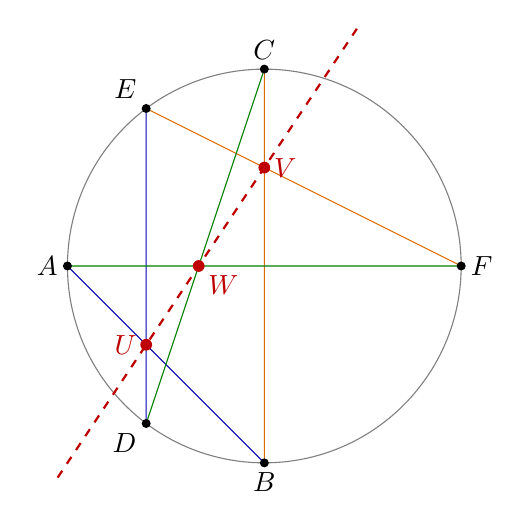
\begin{tikzpicture}[scale=2.5]
	\coordinate (A) at (-1,0);
	\coordinate (B) at (0,-1);
	\coordinate (C) at (0,1);
	\coordinate (D) at (-0.6,-0.8);
	\coordinate (E) at (-0.6,0.8);
	\coordinate (F) at (1,0);
	\draw[gray] (0,0) circle (1);
	\draw[blue!70!black] (A)--(B) (D)--(E);
	\draw[orange!85!black] (B)--(C) (E)--(F);
	\draw[green!50!black] (C)--(D) (F)--(A);
	\draw[red!75!black,thick,dashed] (-1.05,-1.075)--(0.47,1.205);
	\fill (A) circle (0.65pt) node[left]{\(A\)};
	\fill (B) circle (0.65pt) node[below]{\(B\)};
	\fill (C) circle (0.65pt) node[above]{\(C\)};
	\fill (D) circle (0.65pt) node[below left]{\(D\)};
	\fill (E) circle (0.65pt) node[above left]{\(E\)};
	\fill (F) circle (0.65pt) node[right]{\(F\)};
	\fill[red!75!black] (-0.6,-0.4) circle (0.85pt) node[left]{\(U\)};
	\fill[red!75!black] (0,0.5) circle (0.85pt) node[right]{\(V\)};
	\fill[red!75!black] (-0.333333,0) circle (0.85pt) node[below right]{\(W\)};
\end{tikzpicture}

	\caption[Pascal 的六点构形]{Pascal 的六点构形。三组同色的对边分别交于 \(U,V,W\)，红色虚线是它们的公共直线。六点的循环次序允许产生自交边。}
	\label{g1:fig:pascal}
\end{figure}

\cref{g1:fig:pascal}取单位圆上的
\[
	\begin{aligned}
		A&=(-1,0),&\qquad B&=(0,-1),\\
		C&=(0,1),& D&=(-3/5,-4/5),\\
		E&=(-3/5,4/5),& F&=(1,0).
	\end{aligned}
\]
这些点由\cref{g1:exm:circle-parametrization}的参数 \(\infty,-1,1,-2,2,0\) 给出。直线求交得到 \(U=(-3/5,-2/5)\)、\(V=(0,1/2)\)、\(W=(-1/3,0)\)，三点满足 \(y=3x/2+1/2\)。图中六边形虽有自交，关联关系仍然清楚。

\begin{example}[一个交点在无穷远处]\label{g1:exm:pascal-infinity}
	在定理的标准坐标中取 \(d=2\)、\(e=3\)、\(f=-2\)。则
	\[
		U=[-6:0:1],\qquad V=[-6:-6:0],\qquad W=[-8:-2:1].
	\]
	三个点都满足 \(X-Y+6Z=0\)。在仿射图 \(Z=1\) 中，\(BC\) 与 \(EF\) 是平行线，其交点 \(V\) 位于无穷远直线；因此仿射图像中的平行情形已经包含在同一个定理和证明里。
\end{example}

六点两两不同的条件使每条割线都有唯一含义。若相邻点重合，相应的边须改用切线，并要求剩下的交点仍有定义。

\subsection{Brianchon 定理与对偶推导}
\label{g1:subsec:0205:04}

\cref{g1:thm:pascal}涉及曲线上的点、两点连线、两线交点与共线。在对偶平面中，曲线点变成原平面中的切线，连线与交点互换，共线则变成共点。由此得到\term[Brianchondingli]{Brianchon 定理}[Brianchon's theorem]。\footnote{Charles-Julien Brianchon（1783--1864），法国数学家，研究射影几何与圆锥曲线。人物资料见University of St Andrews \href{https://mathshistory.st-andrews.ac.uk/Biographies/Brianchon/}{MacTutor 传记}。}下面逐一写出点、直线与关联关系的对偶对应。

\begin{table}[htbp]
	\centering
	\caption{Pascal 与 Brianchon 构形的对应}
	\label{g1:tab:pascal-brianchon}
	\begin{tabularx}{\textwidth}{@{}XXX@{}}
		\toprule
		Pascal 构形中的对象 & 对偶运算 & Brianchon 构形中的对象 \\
		\midrule
		圆锥曲线上的六点 & 点表示原平面的直线 & 六条不同的曲线切线 \\
		相邻两点的连线 & 张成与相交互换 & 相邻两条切线的交点 \\
		三组对边的交点共线 & 共线与共点互换 & 三条对角线通过公共点 \\
		\bottomrule
	\end{tabularx}
\end{table}

\cref{g1:tab:pascal-brianchon}列出的运算都来自零化子；证明还需要确认六条切线确实落在同一条对偶圆锥曲线上。

\begin{theorem}[Brianchon]\label{g1:thm:brianchon}
	设 \(K=\mathbb R\) 或 \(\mathbb C\)，\(\ell_1,\ldots,\ell_6\) 是 \(\mathbb P^2(K)\) 中一条非退化圆锥曲线的六条两两不同的切线。按循环次序置
	\[
		A=\ell_1\cap\ell_2,\quad B=\ell_2\cap\ell_3,\quad C=\ell_3\cap\ell_4,
		\quad D=\ell_4\cap\ell_5,\quad E=\ell_5\cap\ell_6,\quad F=\ell_6\cap\ell_1.
	\]
	则三条对角线 \(AD,BE,CF\) 共点。
\end{theorem}
\begin{proof}
	把每条 \(\ell_i\) 看作对偶平面中的点 \(L_i\)。由\cref{g1:thm:dual-quadric}，这六个不同的点位于一条非退化对偶圆锥曲线上。该曲线上没有三个不同点共线，这已在\cref{g1:thm:pascal}的证明中由参数二次式说明；由\cref{g1:prop:annihilator-duality}，原平面中的三条不同切线因而不共点。于是所列相邻交点存在，且 \(A\ne D\)、\(B\ne E\)、\(C\ne F\)，各对角线都有定义。

	在对偶平面对 \(L_1,\ldots,L_6\) 使用\cref{g1:thm:pascal}，得到
	\[
		U^*=L_1L_2\cap L_4L_5,\qquad
		V^*=L_2L_3\cap L_5L_6,\qquad
		W^*=L_3L_4\cap L_6L_1
	\]
	共线。直线 \(L_1L_2\) 是原平面中点 \(A\) 的对偶直线，\(L_4L_5\) 是原平面中点 \(D\) 的对偶直线；两条对偶直线的交点 \(U^*\) 因而对应原直线 \(AD\)。同理 \(V^*,W^*\) 分别对应 \(BE,CF\)。包含 \(U^*,V^*,W^*\) 的对偶直线对应原平面的一个点，关联反转保证该点同时属于 \(AD,BE,CF\)，即得结论。
\end{proof}

例如，在实平面取一条圆和一个外切六边形，三条对角线即使看上去没有明显对称性，仍然共点。定理不要求六条切线围成有界的凸区域，公共点也可能位于无穷远处；这些情形与前面允许割线平行的情形相对应。这说明对偶真正保留的是关联及其由线性方程表达的逻辑关系，长度、角度和“内外”都不是推导所需的数据。

% !TeX root = ../../Book1.tex
% 纲要标题：### 2.6 射影映射与参数空间
% 纲要位置：几何学计划纲要.md，第 192 行。
% 正文状态：初稿；尚未正式审核。

% 纲要内容开始
% 
% * Segre 与二次 Veronese 映射的构造
% * Grassmann 空间与 Plücker 坐标
% * 点与超平面的关联簇及其投影
% 
% ---
% 
% 纲要内容结束

\section{射影映射与参数空间}
\label{g1:sec:0206}

圆锥曲线的参数化已经展示过一种变化：把一个点的坐标写成参数的二次式，便把一条射影线放进了另一个射影空间。还可以反过来问：一对射影点、一条直线或一个超平面，能否也用一个射影点来记录？合适的坐标会把“来自同一个对象”的相容条件写成方程，从而让整族几何对象本身成为可以研究的几何集合。本节始终取 \(K=\mathbb R\) 或 \(\mathbb C\)，只用多项式、矩阵秩与坐标图完成这些构造。

\subsection{Segre 与二次 Veronese 映射的构造}
\label{g1:subsec:0206:01}

先考虑两个独立的射影点 \([x_0:\cdots:x_m]\) 和 \([y_0:\cdots:y_n]\)。直接把坐标并排写成 \([x_0:\cdots:x_m:y_0:\cdots:y_n]\) 并不合法：改变第一组的代表而保持第二组不变，通常会改变所得射影点。若改用所有乘积 \(x_i y_j\)，两组代表分别乘以 \(\lambda\) 和 \(\mu\) 时，全部新坐标都乘以同一个 \(\lambda\mu\)。这正是齐次坐标允许的变化。

\begin{definition}[Segre 映射]\label{g1:def:segre-map}
	设 \(K=\mathbb R\) 或 \(\mathbb C\)，\(m,n\ge0\)。映射
	\[
		\sigma_{m,n}:\mathbb P^m(K)\times\mathbb P^n(K)
		\longrightarrow\mathbb P^{(m+1)(n+1)-1}(K),\qquad
		([x],[y])\longmapsto[x_i y_j]_{0\le i\le m,\,0\le j\le n}
	\]
	称为\term[Segreyingshe]{Segre 映射}[Segre map]，目标坐标先按 \(i\)、再按 \(j\) 排列。\footnote{Corrado Segre（1863--1924），意大利数学家，研究高维射影几何、代数曲面和直纹几何。}
\end{definition}

\begin{proposition}[乘积坐标与秩一矩阵]\label{g1:prop:segre-rank-one}
	设 \(K=\mathbb R\) 或 \(\mathbb C\)，\(m,n\ge0\)。Segre 映射良定义且为单射。把目标点的坐标排成 \((m+1)\times(n+1)\) 矩阵 \(Z=(z_{ij})\)，则其像恰由方程
	\[
		z_{ij}z_{k\ell}-z_{i\ell}z_{kj}=0
		\qquad(0\le i,k\le m,\ 0\le j,\ell\le n)
	\]
	给出，也就是所有非零秩一矩阵的射影类。在 \(z_{ab}\ne0\) 的部分，原来两个点可由第 \(b\) 列和第 \(a\) 行恢复。
\end{proposition}
\begin{proof}
	选取非零坐标 \(x_a,y_b\)，则 \(x_a y_b\ne0\)，所以输出坐标不全为零；代表的缩放只产生共同倍数，因而映射良定义。其矩阵是列向量与行向量的乘积 \(Z=xy^{\mathsf T}\)，每个二阶子式均为零。

	反过来，设 \(Z\ne0\) 且全部二阶子式为零，选定 \(z_{ab}\ne0\)。含第 \(a,i\) 行和第 \(b,j\) 列的子式给出
	\[
		z_{ij}=\frac{z_{ib}z_{aj}}{z_{ab}}.
	\]
	因此取 \(x_i=z_{ib}\)、\(y_j=z_{aj}/z_{ab}\)，便有 \(Z=xy^{\mathsf T}\)。这里 \(x_a\ne0\)、\(y_b=1\)，两向量均非零，证明了像的描述。对这样的分解，第 \(b\) 列与 \(x\) 成比例，第 \(a\) 行与 \(y^{\mathsf T}\) 成比例，故它们的射影类唯一，映射为单射。更具体地，在这张坐标图上，逆映射使用的仿射坐标为
	\[
		\frac{x_i}{x_a}=\frac{z_{ib}}{z_{ab}},\qquad
		\frac{y_j}{y_b}=\frac{z_{aj}}{z_{ab}}.
	\]
	分母在所选图上不为零，故这些公式也说明不同图中的恢复结果相容。
\end{proof}

\begin{example}[乘积中的两个方向]\label{g1:exm:segre-fibers}
	取 \(m=n=1\)，则
	\[
		([s:t],[u:v])\longmapsto[su:sv:tu:tv]
	\]
	将 \(\mathbb P^1(K)\times\mathbb P^1(K)\) 一一对应到 \(z_{00}z_{11}-z_{01}z_{10}=0\) 的二次曲面。固定 \([s:t]\) 而改变 \([u:v]\)，像是由 \((s,0,t,0)\)、\((0,s,0,t)\) 张成的射影直线；这两个向量线性无关。固定第二个因子同样得到一条直线。同一族中两条不同直线不相交，因为单射性不允许第一因子或第二因子同时取两个不同值；两族各取一条则恰交于相应有序对的像。\cref{g1:prop:quadric-two-rulings}中的两族直纹，在这里变成了乘积的两个独立方向。
\end{example}

还有另一种坐标构造。若希望把一个点的所有二次表达式同时作为坐标，就应取 \(x_i x_j\) 而不是取两组互不相关的变量。由此得到二次 Veronese 映射。\footnote{Giuseppe Veronese（1854--1917），意大利数学家，研究高维射影几何与几何基础。}

\begin{definition}[二次 Veronese 映射]\label{g1:def:veronese-map}
	设 \(K=\mathbb R\) 或 \(\mathbb C\)，\(n\ge1\)，\(N=\binom{n+2}{2}-1\)。映射
	\[
		\nu_2:\mathbb P^n(K)\longrightarrow\mathbb P^N(K),\qquad
		[x_0:\cdots:x_n]\longmapsto[x_i x_j]_{0\le i\le j\le n}
	\]
	称为\term[Veroneseyingshe]{二次 Veronese 映射}[quadratic Veronese map]。目标坐标按指标 \((i,j)\) 排列，将 \(z_{ij}\) 对称地补成矩阵 \(Z=(z_{ij})\)。
\end{definition}

\begin{proposition}[二次单项式坐标]\label{g1:prop:veronese-image}
	设 \(K=\mathbb R\) 或 \(\mathbb C\)，\(n\ge1\)。二次 Veronese 映射良定义且为单射，其像恰为非零对称秩一矩阵的射影类，亦即对称矩阵 \(Z\) 的所有二阶子式同时为零的射影点集。在 \(z_{aa}\ne0\) 的部分，逆映射由 \(x_i/x_a=z_{ia}/z_{aa}\) 给出。
\end{proposition}
\begin{proof}
	非零向量至少有一个非零坐标 \(x_a\)，故 \(x_a^2\ne0\)；缩放 \(x\) 使全部二次单项式乘以相同的平方倍数。这证明良定义，且像矩阵 \(xx^{\mathsf T}\) 为对称秩一矩阵。

	设对称矩阵 \(Z\ne0\) 的所有二阶子式均为零。必有某个对角元 \(z_{aa}\ne0\)：否则对任意 \(i,j\)，主子式 \(z_{ii}z_{jj}-z_{ij}^2=0\) 会强迫 \(z_{ij}=0\)，与 \(Z\ne0\) 矛盾。令 \(x_i=z_{ia}/z_{aa}\)，于是 \(x_a=1\)，而子式关系给出
	\[
		\frac{z_{ij}}{z_{aa}}
		=\frac{z_{ia}}{z_{aa}}\frac{z_{ja}}{z_{aa}}=x_i x_j.
	\]
	所以 \([Z]=[xx^{\mathsf T}]\)，并且上述比值唯一恢复 \([x]\)。这同时证明了像的描述、单射性及逆坐标公式。
\end{proof}

在实数情形，上一证明没有要求 \(z_{aa}\) 有实平方根。因为讨论的是矩阵的射影类，可以先把整个矩阵除以 \(z_{aa}\)；这也解释了为什么负半定的秩一矩阵仍表示像中的点。当 \(n=1\) 时，\(\nu_2([s:t])=[s^2:st:t^2]\)，正是前一节的圆锥曲线参数化。当 \(n=2\) 时，得到 \(\mathbb P^5(K)\) 中的 Veronese 曲面。

\ProseParagraphBreak

这两种映射还有一个直接用途：使原来的高次方程成为新空间的线性方程。例如任意二次齐次式 \(q(x)=\sum_{i\le j}c_{ij}x_i x_j\) 都满足
\[
	q(x)=0\quad\Longleftrightarrow\quad
	\sum_{i\le j}c_{ij}z_{ij}=0\quad\text{在 }[z]=\nu_2([x])\text{ 上成立}.
\]
右边是一个超平面与 Veronese 像的相交条件。同样，双线性关系 \(\sum a_{ij}x_i y_j=0\) 经 Segre 映射成为超平面截面。目标空间中的子式关系刻画了哪些射影点属于这些映射的像。这些模型的代数几何推广可参看\cite[第I章, 第2, Exercises节 2.12--2.15]{Hartshorne1977}。

\subsection{Grassmann 空间与 Plücker 坐标}
\label{g1:subsec:0206:02}

射影空间以一维向量子空间为点。若把“维数一”换成“维数 \(k\)”，同样得到一个值得研究的对象集合。困难在于：一个子空间有许多组基，把基向量的坐标直接抄下来会记录过多的选择。行列式恰能把换基的影响压缩成一个共同倍数。

\begin{definition}[Grassmann 空间]\label{g1:def:grassmannian}
	设 \(K=\mathbb R\) 或 \(\mathbb C\)，\(V\) 为 \(n\) 维 \(K\)-向量空间，\(1\le k\le n\)。所有 \(k\) 维向量子空间组成的集合
	\[
		\operatorname{Gr}(k,V)=\{\,W\subseteq V:W\text{ 为向量子空间且 }\dim_K W=k\,\}
	\]
	称为\term[Grassmannkongjian]{Grassmann 空间}[Grassmannian]，当 \(V=K^n\) 时也记为 \(\operatorname{Gr}(k,n;K)\)。\footnote{Hermann Günter Grassmann（1809--1877），德国数学家，发展了向量运算和外代数，并以坐标研究不同维数的子空间。}
	\symidx{\(\operatorname{Gr}(k,V)\)：Grassmann 空间}
\end{definition}

这里的 \(k,n\) 都是向量空间维数；\(W\) 对应 \(\mathbb P(V)\) 中的 \((k-1)\) 维射影子空间。特别地，\(\operatorname{Gr}(1,V)=\mathbb P(V)\)，而 \(\operatorname{Gr}(2,4;K)\) 参数化射影三维空间中的所有直线。先把后一情形具体写出。选取二维子空间的有序基 \(u,v\)，将它们写成矩阵的两行，并定义六个子式
\[
	p_{ij}=u_i v_j-u_j v_i\qquad(1\le i<j\le4).
\]
它们称为该直线的\term[Pluckerzuobiao]{Plücker 坐标}[Plücker coordinates]。\footnote{Julius Plücker（1801--1868），德国数学家和物理学家，研究解析几何、直线几何及光谱。}矩阵的秩为 \(2\)，故至少一个二阶子式非零。若将有序基替换为 \((u',v')^{\mathsf T}=S(u,v)^{\mathsf T}\)，其中 \(S\in\operatorname{GL}_2(K)\)，每个子式都乘以 \(\det S\)，所以射影点 \([p_{12}:p_{13}:p_{14}:p_{23}:p_{24}:p_{34}]\) 与基的选择无关。

\begin{theorem}[射影三维空间中直线的坐标]\label{g1:thm:plucker-gr24}
	设 \(K=\mathbb R\) 或 \(\mathbb C\)。Plücker 坐标给出 \(\operatorname{Gr}(2,4;K)\) 到 \(\mathbb P^5(K)\) 的单射，其像恰为二次曲面
	\begin{equation}\label{g1:eq:plucker-gr24}
		p_{12}p_{34}-p_{13}p_{24}+p_{14}p_{23}=0.
	\end{equation}
	在 \(p_{12}\ne0\) 的部分，每个子空间有唯一的行基矩阵
	\[
		\begin{pmatrix}
			1&0&a&b\\
			0&1&c&d
		\end{pmatrix},
	\]
	其中 \(a,b,c,d\in K\) 可任意取值，相应射影坐标为 \([1:c:d:-a:-b:ad-bc]\)。
\end{theorem}
\begin{proof}
	先说明关系式从何而来。将 \(p_{ij}=u_i v_j-u_j v_i\) 代入左边，展开得
	\[
		\begin{aligned}
			&(u_1v_2-u_2v_1)(u_3v_4-u_4v_3)\\
			&\quad-(u_1v_3-u_3v_1)(u_2v_4-u_4v_2)\\
			&\quad+(u_1v_4-u_4v_1)(u_2v_3-u_3v_2)=0;
		\end{aligned}
	\]
	每个含两个 \(u\) 坐标和两个 \(v\) 坐标的单项式出现两次且符号相反。这证明必要性。

	若 \(p_{12}\ne0\)，基矩阵的前两列组成可逆矩阵 \(C\)。将整矩阵左乘 \(C^{-1}\)，得到所述行基矩阵，而且前两坐标为 \((1,0)\)、\((0,1)\) 的两行在该子空间中唯一。逐项计算子式即得 \((1,c,d,-a,-b,ad-bc)\)。反过来，对满足关系式且 \(p_{12}\ne0\) 的射影点，将全部坐标除以 \(p_{12}\)，记归一化后的坐标为 \(\widetilde p_{ij}\)。取
	\[
		a=-\widetilde p_{23},\quad b=-\widetilde p_{24},\quad
		c=\widetilde p_{13},\quad d=\widetilde p_{14}.
	\]
	对应行基矩阵的前五个子式就是指定坐标；第六个由
	\[
		ad-bc=\widetilde p_{13}\widetilde p_{24}
		-\widetilde p_{14}\widetilde p_{23}=\widetilde p_{34}
	\]
	保证一致。这给出了存在性，也说明相同坐标只能恢复同一个子空间。

	任意非零六元组都有某个 \(p_{ij}\ne0\)。交换坐标轴可使这对指标成为 \(1,2\)。这里交换时同时使用 \(p_{ji}=-p_{ij}\)；关系式的左边在交换任意相邻两个指标时只改变符号，故它的零条件保持不变。于是上述构造适用于每一张图，并在图的重叠处由恢复出的子空间的唯一性相容，证明全局结论。
\end{proof}

\begin{example}[由六个数恢复一条直线]\label{g1:exm:plucker-reconstruction}
	在 \(K=\mathbb R\) 或 \(\mathbb C\) 上，六元组 \([1:2:3:4:5:-2]\) 满足 \(-2-10+12=0\)。按\cref{g1:thm:plucker-gr24}，其二维子空间有行基
	\[
		u=(1,0,-4,-5),\qquad v=(0,1,2,3),
	\]
	故对应直线为 \([s:t:-4s+2t:-5s+3t]\)，其中 \([s:t]\in\mathbb P^1(K)\)。若把最后一个坐标改成 \(0\)，关系式左边变成 \(2\)，所得射影点便不代表任何直线。所以六个齐次坐标之间的二次关系是实质约束。
\end{example}

一般的 \(\operatorname{Gr}(k,n;K)\) 也有同样可操作的坐标。将一组基写成秩为 \(k\) 的 \(k\times n\) 矩阵 \(M\)，选择一个非零的 \(k\) 阶子式。若它来自前 \(k\) 列，左乘这 \(k\) 列组成的矩阵的逆，即得唯一形式
\[
	M=[I_k\mid Z],\qquad Z\in\operatorname{Mat}_{k\times(n-k)}(K).
\]
唯一性的理由是：若 \(S[I_k\mid Z]=[I_k\mid Z']\)，比较前 \(k\) 列便有 \(S=I_k\)，继而 \(Z=Z'\)。任意 \(Z\) 都给出秩为 \(k\) 的矩阵。因此，这一部分中的子空间可用 \(k(n-k)\) 个自由参数描述。其他非零子式给出其他图；在重叠处，变换是先选出新的可逆子矩阵 \(C\)，再作 \(C^{-1}M\)。逆矩阵的余子式公式说明，新参数是旧参数的有理函数，分母就是被假设非零的 \(\det C\)。

\ProseParagraphBreak

所有 \(k\) 阶子式在换基时仍同乘 \(\det S\)，故又给出一个射影点，落在 \(\mathbb P^{\binom nk-1}(K)\) 中。这些坐标确实能恢复子空间：在选定子式归一化为 \(1\) 后， \([I_k\mid Z]\) 中的每个 \(Z_{ij}\) 都是用相应外部列替换第 \(i\) 个单位列所得子式，至多差一个由列排序产生的符号。因此所得到的射影映射为单射。一般维数时子式之间还有一组二次关系；式\eqref{g1:eq:plucker-gr24}给出了其中最小的非平凡模型。这里的参数数目由坐标图中的自由参数直接给出。

\subsection{点与超平面的关联簇及其投影}
\label{g1:subsec:0206:03}

对偶空间把一个超平面视为一个点；若同时保留原空间中的点，就能把“点属于超平面”本身作为一个几何对象。设 \(V=K^{n+1}\)、\(n\ge1\)。对偶空间 \(V^*\) 是 \(V\) 上的线性函数全体，非零函数 \(\alpha\) 的核给出超平面 \(\mathbb P(\ker\alpha)\)。定义
\[
	\mathcal I_n=
	\{\,([x],[\alpha])\in\mathbb P(V)\times\mathbb P(V^*):\alpha(x)=0\,\},
\]
称为点与超平面的\term[guanliancu]{关联簇}[incidence variety]。这里先将“簇”理解为这组方程给出的几何集合，关于代数簇的结构与一般性质将在第五卷中系统建立。在对偶基下，若 \(\alpha\) 的坐标为 \((a_0,\ldots,a_n)\)，其方程就是
\[
	\sum_{i=0}^n a_i x_i=0.
\]
分别缩放 \(a\) 和 \(x\) 不改变零条件，所以定义与代表选择无关。

\begin{proposition}[关联集合的两个投影]\label{g1:prop:incidence-fibers}
	设 \(K=\mathbb R\) 或 \(\mathbb C\)，\(V=K^{n+1}\)、\(n\ge1\)，并记 \(\mathcal I_n=\{([x],[\alpha])\in\mathbb P(V)\times\mathbb P(V^*):\alpha(x)=0\}\)。从 \(\mathcal I_n\) 到 \(\mathbb P(V)\)、\(\mathbb P(V^*)\) 的坐标投影都为满射。固定 \([x]\) 后，其上方的集合是 \(\mathbb P(\{\alpha:\alpha(x)=0\})\)，固定 \([\alpha]\) 后，其上方的集合是 \(\mathbb P(\ker\alpha)\)；二者都同构于 \(\mathbb P^{n-1}(K)\)。经 Segre 映射，\(\mathcal I_n\) 恰成为 Segre 像与超平面 \(\sum_i z_{ii}=0\) 的交集。
\end{proposition}
\begin{proof}
	固定非零向量 \(x\)，线性映射 \(V^*\rightarrow K\)、\(\alpha\mapsto\alpha(x)\) 是满射：将 \(x\) 扩为一组基，令线性函数在 \(x\) 上取值 \(1\)、在其余基向量上取值 \(0\) 即可。其核因而为 \(n\) 维，非零核向量的射影类就是所有经过 \([x]\) 的超平面。固定非零 \(\alpha\) 时，\(\alpha:V\rightarrow K\) 也满射，所以 \(\ker\alpha\) 同样为 \(n\) 维。由于 \(n\ge1\)，这些核都含非零向量，故两个投影都满射。最后，Segre 坐标取 \(z_{ij}=x_i a_j\) 时，关联方程恰为 \(\sum_i z_{ii}=0\)。\cref{g1:prop:segre-rank-one}给出的单射性和逆映射保证此描述没有额外或遗漏的点。
\end{proof}

分别记这两个投影为 \(\pi_1([x],[\alpha])=[x]\)、\(\pi_2([x],[\alpha])=[\alpha]\)。

\begin{figure}[htbp]
	\centering
	% !TeX root = ../Book1.tex
\begin{tikzcd}[column sep=large,row sep=large]
	& \mathcal I_n \arrow[dl, "\pi_1"'] \arrow[dr, "\pi_2"] & \\
	\mathbb P(V) && \mathbb P(V^*)
\end{tikzcd}

	\caption[点与超平面的关联]{点与超平面的关联。左边一个点的上方记录所有经过它的超平面；右边一个超平面的上方记录其全部点。}
	\label{g1:fig:incidence-projections}
\end{figure}

\cref{g1:fig:incidence-projections}把同一个条件的两种读法并排呈现。当 \(n=2\) 时，固定点得到过该点的直线束，固定直线得到这条直线上的点列；当 \(n=1\) 时，两边的纤维都是一个点，因为射影直线上的超平面本身就是点。这里映射的\term[xianwei]{纤维}[fiber]指一个指定点的逆像。

\ProseParagraphBreak

这些方程也解释了关联为什么是射影不变量。若 \(g\in\operatorname{GL}(V)\)，同时变换
\[
	[x]\longmapsto[gx],\qquad [\alpha]\longmapsto[\alpha\circ g^{-1}],
\]
则 \((\alpha\circ g^{-1})(gx)=\alpha(x)\)。因此点属于超平面的条件在改变射影坐标后保持不变。这些模型提出了三个共同问题：哪些条件描述的是一个子空间而非某组基，哪些参数变化只改变描述而不改变对象，哪些局部坐标能覆盖整个对象族。本节的秩一分解、子式恢复和关联方程已经分别给出了可直接计算的答案。后续研究更一般的曲线、曲面和参数空间时，这三个问题仍然存在。


\begin{chaptersummary}
	射影空间的点是一维向量子空间，仿射图是把一个非零坐标归一为 \(1\) 后得到的坐标区域。子空间的关联因此还原为线性代数，标架则把代表向量的相对比例一并固定。射影线上三个点可以完全归一化，第四个点留下交比；排列四点会改变这个值，故不变量必须与有序或无序对象的选择相对应。

	\ProseParagraphBreak

	二次多项式先分离能由平移消去的线性项与核中的障碍，再依允许的变换选择 Euclid 或仿射标准形。齐次化将二次项、线性项和常数项放进一个矩阵，但同时必须保留仿射图，才能恢复原来的仿射对象。实射影分类需要惯性，复射影分类只需秩；实零点集相同并不保证二次方程等价。曲面中的线性子空间由全迷向子空间控制，两个直纹族则把这套线性代数变成可见的几何。

	\ProseParagraphBreak

	对偶空间本来就把超平面参数化，非退化配对进一步为每个点指定一个极超平面。在二次曲面上，这个超平面恰是切超平面；配对退化时，对应可能失去定义或唯一性。圆锥曲线的有理参数把六点构造化成可检查的坐标等式，对偶再给出六条切线的共点结论。乘积、二次单项式、子空间坐标与关联方程展示了同一种构造方法：先记录几何对象所决定的坐标，证明选择无关，再说明哪些方程刻画像，并在局部坐标中恢复原对象。
\end{chaptersummary}

\BookExercises

\begin{exercise}\label{g1:ex:projective-completion}
	在 \(\mathbb R^2\) 中，将直线 \(2x-y=1\) 与 \(2x-y=3\) 补全到 \(\mathbb P^2(\mathbb R)\)。求其交点，并在以 \(X_1\ne0\) 为条件的图中写出交点坐标。解释为什么它在这张图中不是无穷远点。
\end{exercise}
\begin{solution}
	采用 \(x=X_1/X_0,y=X_2/X_0\)，补全方程为 \(2X_1-X_2=X_0\)、\(2X_1-X_2=3X_0\)。相减得 \(X_0=0\)，继而 \(X_2=2X_1\)，故唯一交点为 \([0:1:2]\)。在图 \(X_1\ne0\) 中取坐标 \((X_0/X_1,X_2/X_1)\)，交点坐标为 \((0,2)\)。原图的无穷远条件为 \(X_0=0\)，新图的无穷远条件则是 \(X_1=0\)。同一点可在一张图之外而在另一张图之内，所以“无穷远”描述的是相对于图的位置。
\end{solution}

\begin{exercise}\label{g1:ex:projective-frame}
	求把 \([e_0],[e_1],[e_2],[1:1:1]\) 依次送到 \([1:1:0],[0:1:1],[1:0:1],[4:3:5]\) 的射影变换，并求它把 \([1:2:-1]\) 送到哪里。
\end{exercise}
\begin{solution}
	取前三个像的代表 \(v_0=(1,1,0),v_1=(0,1,1),v_2=(1,0,1)\)。其列矩阵行列式为 \(2\)，故组成基。由 \(a_0v_0+a_1v_1+a_2v_2=(4,3,5)\)，解得 \((a_0,a_1,a_2)=(1,2,3)\)，均非零，故所给像也构成标架。依\cref{g1:thm:projective-frame}的构造，变换的矩阵可取
	\[
		M=\begin{pmatrix}1&0&3\\1&2&0\\0&2&3\end{pmatrix}.
	\]
	它将最后一个代表送到 \((4,3,5)\)，且 \(\det M=12\ne0\)。计算 \(M(1,2,-1)^{\mathsf T}=(-2,5,1)^{\mathsf T}\)，故所求像为 \([-2:5:1]\)。若只把 \(v_i\) 原样作为列，前三个像虽然正确，第四个像却不正确；列的相对比例正是第四点所确定的数据。
\end{solution}

\begin{exercise}\label{g1:ex:cross-ratio-test}
	在实射影线上，判断有序四点 \((\infty,0,1,3)\) 与 \((2,0,1,3/2)\) 是否射影等价。若等价，给出唯一变换。再判断把第二组的最后一点改成 \(4\) 后是否仍然等价。
\end{exercise}
\begin{solution}
	把前三点 \(\infty,0,1\) 送到 \(2,0,1\) 的分式为 \(f(t)=2t/(t+1)\)，齐次矩阵为 \(\begin{pmatrix}2&0\\1&1\end{pmatrix}\)，行列式非零。它满足 \(f(3)=3/2\)，所以第一组与原第二组等价；由前三点构成标架知变换唯一。改成 \(4\) 后，同一个唯一候选变换不能匹配第四点，故不等价。也可直接检查：\((2,0;1,3/2)=3\)，而 \((2,0;1,4)=-2\)，与原交比 \(3\) 不同。
\end{solution}

\begin{exercise}\label{g1:ex:affine-projective-group}
	设 \(K=\mathbb R\) 或 \(\mathbb C\)，\(n\geq1\)。证明 \(\mathbb P^n(K)\) 的射影变换保持超平面 \(X_0=0\) 当且仅当它在图 \(X_0\ne0\) 上的限制是仿射同构。说明每个仿射同构都有唯一这样的射影扩充。
\end{exercise}
\begin{solution}
	将线性代表分块写为 \(M=\begin{pmatrix}a&\ell\\b&S\end{pmatrix}\)。若保持 \(X_0=0\)，则对所有 \(x\in K^n\) 都有 \(\ell x=0\)，故 \(\ell=0\)。由于 \(M\) 可逆，\(a\ne0\)、\(S\) 可逆；除以 \(a\) 后，矩阵形如 \(\begin{pmatrix}1&0\\b'&S'\end{pmatrix}\)，在仿射图中诱导 \(x\mapsto b'+S'x\)。

	反过来，任给仿射同构 \(x\mapsto b'+S'x\)，所写块矩阵可逆，并保持 \(X_0=0\)，给出扩充。若已有射影变换在整个图上的限制为该仿射同构，那么图被双射到自身，其补集也被保持，所以其代表可归一化为同一种块矩阵。仿射函数的常数项与线性部分唯一，故扩充唯一。这里先说明限制在整个图上存在；仅在图中某个小区域看到分式表达式，并不能直接套用结论。
\end{solution}

\begin{exercise}
	\label{g1:ex:quadric-center-axes}
	在通常 Euclid 空间 \(\mathbb R^3\) 中考虑
	\[
		2x^2+2xy+2y^2+4x-2y+z^2+4=0.
	\]
	求中心、正交标准形和各半轴长，并求其齐次化矩阵的秩与惯性。
\end{exercise}
\begin{solution}
	二次项矩阵和线性系数列为
	\[
		A=\begin{pmatrix}2&1&0\\1&2&0\\0&0&1\end{pmatrix},
		\qquad b=(2,-1,0)^{\mathsf T}.
	\]
	由\cref{g1:prop:quadric-center}，中心满足 \(2x+y=-2\)、\(x+2y=1\)、\(z=0\)，所以唯一中心为 \(a=(-5/3,4/3,0)\)。在中心处，利用 \(Aa=-b\)，有
	\[
		F(a)=a^{\mathsf T}Aa+2b^{\mathsf T}a+4
		=b^{\mathsf T}a+4=-\frac23.
	\]
	矩阵 \(A\) 在单位方向 \((1,1,0)/\sqrt2\)、\((1,-1,0)/\sqrt2\)、\((0,0,1)\) 上的特征值分别为 \(3,1,1\)。因此令
	\[
		U=\frac{x+y+1/3}{\sqrt2},\qquad
		V=\frac{x-y+3}{\sqrt2},\qquad W=z,
	\]
	得到 \(3U^2+V^2+W^2=2/3\)。这是椭球面，半轴长分别为 \(\sqrt2/3\)、\(\sqrt{2/3}\)、\(\sqrt{2/3}\)，后两条轴可以在它们张成的平面内作任意正交选择。

	齐次化矩阵合同于 \(\operatorname{diag}(-2/3,A)\)，因为平移到中心已经消去了全部线性项。故其秩为 \(4\)，惯性为 \((3,1,0)\)。这项结论同时说明该射影曲面没有实射影直线。
\end{solution}

\begin{exercise}
	\label{g1:ex:paraboloid-parameter}
	对 \(t\in\mathbb R\)，在 \(\mathbb R^3\) 中令
	\[
		F_t(x,y,z)=x^2+z^2+2ty-1.
	\]
	\begin{enumerate}
		\item 求 \(F_t\) 的中心集、其零点集的形状，以及齐次化的秩与惯性。
		\item 对 \(s,t\ne0\)，证明方程 \(F_s=0\) 与 \(F_t=0\) 总是仿射等价，而 Euclid 等价当且仅当 \(|s|=|t|\)。
	\end{enumerate}
\end{exercise}
\begin{solution}
	1. 二次项矩阵为 \(\operatorname{diag}(1,0,1)\)，核为 \(y\) 轴，线性项的系数列是 \((0,t,0)\)。当 \(t=0\) 时，中心是整条 \(y\) 轴，零点集为圆柱面 \(x^2+z^2=1\)，中心值为 \(-1\)。由\cref{g1:prop:homogenized-rank}，齐次化的秩为 \(3\)，惯性为 \((2,1,1)\)。当 \(t\ne0\) 时没有中心。令 \(Y=y-1/(2t)\)，方程成为 \(x^2+z^2+2tY=0\)，所以是以 \(y\) 方向为轴的抛物面；其齐次化的秩为 \(4\)，惯性为 \((3,1,0)\)。

	2. 对 \(s,t\ne0\)，变换 \((x,y,z)\mapsto(x,(t/s)y,z)\) 使 \(F_s\) 变为 \(F_t\)，故方程仿射等价。Euclid 标准形中的非零特征值为 \(\{1,1\}\)，剩余线性项长度为 \(|t|\)。若两个方程 Euclid 等价，还可以有整体倍数 \(\mu\ne0\)；二次项的特征值必须满足 \(\{1,1\}=\{\mu,\mu\}\)，故 \(\mu=1\)，再由\cref{g1:thm:euclidean-quadric-normal}得到 \(|s|=|t|\)。反过来，\(s=t\) 时取恒等变换，\(s=-t\) 时取 \(y\mapsto-y\) 的反射，均给出 Euclid 等价。
\end{solution}

\begin{exercise}
	\label{g1:ex:quadric-locus-information}
	在 \(\mathbb R^3\) 中令 \(F=x^2+y^2\)、\(G=x^2+4y^2\)。证明它们的零点集相同，但作为方程不 Euclid 等价；再给出一个保持这个共同零点集、却不把 \(G\) 变成自身非零倍数的 Euclid 变换。
\end{exercise}
\begin{solution}
	因为每一项都非负，两个方程都等价于 \(x=y=0\)，故实零点集都是 \(z\) 轴。两者有中心，中心值都为零；二次项的非零特征值多重集分别为 \(\{1,1\}\) 和 \(\{1,4\}\)。方程 Euclid 等价要求存在非零 \(\mu\)，使 \(\{\mu,\mu\}=\{1,4\}\)，这是不可能的。因此相同实点集不能恢复 Euclid 方程类别。

	取绕 \(z\) 轴的正交变换
	\[
		(x,y,z)\longmapsto
		\left(\frac{x-y}{\sqrt2},\frac{x+y}{\sqrt2},z\right).
	\]
	它固定整条 \(z\) 轴，而变换后的 \(G\) 为
	\[
		\frac{(x-y)^2}{2}+2(x+y)^2
		=\frac52x^2+3xy+\frac52y^2.
	\]
	新出现的交叉项表明它不是 \(G\) 的非零倍数。这说明点集的对称群可以严格大于指定二次方程的对称群。
\end{solution}

\begin{exercise}
	\label{g1:ex:isotropic-graph-orthogonal}
	在 \(\mathbb R^5=\mathbb R^2\oplus\mathbb R^2\oplus\mathbb R\) 上考虑
	\[
		q(u,v,z)=\lVert u\rVert^2-\lVert v\rVert^2.
	\]
	证明它的每个极大全迷向子空间都唯一写成
	\[
		U_T=\{\,(u,Tu,z):u\in\mathbb R^2,\ z\in\mathbb R\,\},
		\qquad T\in O(2).
	\]
	据此说明对应射影二次曲面的极大射影平面都经过哪一个点。
\end{exercise}
\begin{solution}
	该型的惯性为 \((2,2,1)\)，根基为 \(R=\{(0,0,z)\}\)。由\cref{g1:thm:quadric-linear-dimension}，极大全迷向子空间 \(U\) 维数为 \(3\)，并包含 \(R\)。将它投影到前四个坐标，得到二维全迷向子空间 \(W\)，且 \(U=W\oplus R\)。

	从 \(W\) 到第一个 \(\mathbb R^2\) 的投影单射：若 \(u=0\)，则 \(q=0\) 迫使 \(v=0\)。由于两边都是二维，这个投影也是满射，故恰有一个线性映射 \(T\) 使 \(W=\{(u,Tu)\}\)。全迷向条件给出 \(\lVert Tu\rVert^2=\lVert u\rVert^2\) 对所有 \(u\) 成立。用实内积的极化公式可得 \(\langle Tu,Tw\rangle=\langle u,w\rangle\)，即 \(T^{\mathsf T}T=I\)。因此 \(T\in O(2)\)，且其唯一性来自图像对每个 \(u\) 的唯一取值。

	反过来，任意正交 \(T\) 都使 \(q\) 在 \(U_T\) 上恒为零；\(U_T\) 维数为 \(3\)，已经达到最大值，故极大。射影化后得到全部极大射影平面，它们都包含根基对应的点 \([0:0:0:0:1]\)。
\end{solution}

\begin{exercise}
	\label{g1:ex:quadric-cone-family}
	在 \(\mathbb P^3(\mathbb R)\) 中考虑参数族
	\[
		Q_t:\ X_0X_3-X_1^2-tX_2^2=0.
	\]
	\begin{enumerate}
		\item 按 \(t\) 的符号求秩、惯性和最大射影线性子空间维数。
		\item 当 \(t=0\) 时，证明曲面中的全部射影直线恰为
		\[
			L_{[a:b]}=\mathbb P\!\left(
			\operatorname{span}\bigl((a^2,ab,0,b^2),(0,0,1,0)\bigr)\right),
			\quad [a:b]\in\mathbb P^1(\mathbb R).
		\]
	\end{enumerate}
\end{exercise}
\begin{solution}
	1. 乘积 \(X_0X_3\) 贡献一个正方向、一个负方向；\(-X_1^2\) 贡献一个负方向。因此 \(t>0\) 时惯性为 \((1,3,0)\)，秩为 \(4\)，最大全迷向维数为 \(1\)，曲面内最大射影线性子空间只是点，没有实直线。\(t<0\) 时惯性为 \((2,2,0)\)，秩为 \(4\)，最大射影线性子空间维数为 \(1\)；由射影分类及\cref{g1:prop:quadric-two-rulings}，有两个直纹族。\(t=0\) 时惯性为 \((1,2,1)\)，秩为 \(3\)，最大射影线性维数仍为 \(1\)。

	2. 在 \(t=0\) 时，根基由 \(e_2=(0,0,1,0)\) 张成。任意曲面内直线对应一个二维全迷向子空间，已经达到最大维数，所以包含根基。模去根基后，它由 \((X_0,X_1,X_3)\ne0\) 且 \(X_0X_3=X_1^2\) 的一个射影点决定。若 \(X_0\ne0\)，把该点写为 \([1:u:u^2]\)，对应 \([a:b]=[1:u]\)；若 \(X_0=0\)，则 \(X_1=0\)、\(X_3\ne0\)，对应 \([a:b]=[0:1]\)。这给出全部且唯一的参数点。

	对每个 \([a:b]\)，向量 \((a^2,ab,0,b^2)\) 非零、迷向，且不在根基中；它与根基向量的所有配对为零。因此所列二维空间全迷向，其射影化确为曲面内直线。全部直线都经过顶点 \([0:0:1:0]\)，与满秩分裂曲面的两个直纹族有不同的相交关系。
\end{solution}

\begin{exercise}
	\label{g1:ex:complex-line-real-sphere}
	考虑复射影二次曲面
	\[
		Q:\ X_1^2+X_2^2+X_3^2-X_0^2=0
		\quad\text{于 }\mathbb P^3(\mathbb C).
	\]
	证明 \(u=(0,1,i,0)\)、\(v=(1,0,0,1)\) 张成的二维复子空间给出 \(Q\) 中的一条复射影直线，求它上面的全部实射影点，并解释这为何不与实球面没有实直线矛盾。
\end{exercise}
\begin{solution}
	分别计算得到 \(q(u)=1+i^2=0\)、\(q(v)=1-1=0\)，且对应双线性型满足 \(B(u,v)=0\)。所以对任意复数 \(a,b\)，
	\[
		q(au+bv)=a^2q(u)+2abB(u,v)+b^2q(v)=0.
	\]
	\(u,v\) 线性无关，故其张成空间二维，射影化是一条复直线。该直线的点写成 \([b:a:ia:b]\)。若 \(b\ne0\)，归一化为 \([1:w:iw:1]\)，它有实代表当且仅当 \(w\) 与 \(iw\) 同时为实数，故 \(w=0\)。若 \(b=0\)，唯一射影点为 \([0:1:i:0]\)，没有实代表。因此直线只有一个实点 \([1:0:0:1]\)。

	实射影直线须由二维实向量子空间射影化而来，包含无穷多个实点；本例的二维空间是复空间，不能据此推出存在二维实全迷向子空间。实型的惯性为 \((3,1,0)\)，仍由\cref{g1:thm:quadric-linear-dimension}排除实射影直线。
\end{solution}

\begin{exercise}\label{g1:ex:polarity-coordinate-change}
	设 \(K=\mathbb R\) 或 \(\mathbb C\)，\(A\) 为可逆对称矩阵。在旧坐标中，二次曲面为 \(x^{\mathsf T}Ax=0\)。改用 \(x=Sy\)，其中 \(S\) 可逆。求新坐标中的二次型矩阵、极超平面系数和对偶二次型矩阵，并解释为什么对点和超平面的坐标不能使用同一个变换公式。
\end{exercise}
\begin{solution}
	直接代入得到新矩阵 \(A'=S^{\mathsf T}AS\)。旧超平面 \(a^{\mathsf T}x=0\) 变成 \((S^{\mathsf T}a)^{\mathsf T}y=0\)，故新系数为 \(a'=S^{\mathsf T}a\)。若旧点为 \(x\)，新点为 \(y=S^{-1}x\)，其极超平面的新系数为
	\[
		A'y=S^{\mathsf T}ASS^{-1}x=S^{\mathsf T}Ax,
	\]
	恰与先在旧坐标取极超平面再变换一致。对偶方程的新矩阵是
	\[
		(A')^{-1}=S^{-1}A^{-1}S^{-\mathsf T}.
	\]
	这是因为旧系数 \(a=S^{-\mathsf T}a'\)，将其代入旧对偶方程便得到同一矩阵。点的坐标用 \(S^{-1}\)，超平面系数用 \(S^{\mathsf T}\)；它们必须保持求值 \(a^{\mathsf T}x=(a')^{\mathsf T}y\)，不能因都是坐标列而使用相同规则。
\end{solution}

\begin{exercise}\label{g1:ex:ellipse-tangents}
	在实仿射平面中考虑椭圆 \(x^2/9+y^2/4=1\)。用对偶二次曲面的方法，求从点 \((6,0)\) 引出的全部实切线及其切点。再解释为什么从原点引不出实切线。
\end{exercise}
\begin{solution}
	齐次方程为 \(4X^2+9Y^2-36Z^2=0\)。由\cref{g1:thm:dual-quadric}，直线系数 \([a:b:c]\) 对应切线的充要条件是 \(9a^2+4b^2-c^2=0\)。过 \([6:0:1]\) 的条件为 \(c=-6a\)，于是 \(4b^2=27a^2\)。这里 \(a\ne0\)，否则三个系数全零。按比例取 \(a=2\)，得到两条直线
	\[
		2x+3\sqrt3\,y=12,\qquad 2x-3\sqrt3\,y=12.
	\]
	矩阵逆像给出切点的齐次代表
	\[
		\operatorname{diag}(1/4,1/9,-1/36)
		\begin{pmatrix}2\\ \pm3\sqrt3\\ -12\end{pmatrix}
		=\begin{pmatrix}1/2\\ \pm\sqrt3/3\\ 1/3\end{pmatrix},
	\]
	故切点为 \((3/2,\pm\sqrt3)\)，分别代入椭圆和相应直线均成立。过原点则 \(c=0\)，对偶方程成为 \(9a^2+4b^2=0\)。在实数域上只能有 \(a=b=0\)，不是合法直线系数，故没有实切线。
\end{solution}

\begin{exercise}\label{g1:ex:cone-dual-fibers}
	在 \(\mathbb P^3(K)\)、\(K=\mathbb R\) 或 \(\mathbb C\) 中，令 \(Q\) 由 \(XZ-Y^2=0\) 定义。求全部光滑点处切平面组成的对偶点集，并求每一个切平面对应的全部切点。
\end{exercise}
\begin{solution}
	配对的根基为 \(K(0,0,0,1)\)，因此唯一非光滑点是顶点 \(O=[0:0:0:1]\)。在其余点 \([X:Y:Z:W]\)，切平面系数可取 \([Z:-2Y:X:0]\)。故若对偶坐标写成 \([a:b:c:d]\)，像满足
	\[
		d=0,\qquad b^2-4ac=0.
	\]
	反过来，任一满足这些方程的射影点都有 \((a,b,c)\ne(0,0,0)\)，点 \([2c:-b:2a:w]\) 对每个 \(w\in K\) 都位于 \(Q\setminus\{O\}\)，且切平面正是 \([a:b:c:0]\)。若一个点给出同一切平面，存在 \(\lambda\ne0\) 使 \((Z,-2Y,X)=\lambda(a,b,c)\)，缩放其代表向量后便是上述形式。因此每个切平面的全部切点是一条经过顶点的射影直线去掉顶点。对偶像是超平面 \(d=0\) 内的一条非退化圆锥曲线；不同母线被区分，而同一母线上各光滑点被合并。
\end{solution}

\begin{exercise}\label{g1:ex:five-conic-points}
	在 \(K=\mathbb R\) 或 \(\mathbb C\) 上，取标准圆锥曲线 \(XZ-Y^2=0\) 的参数 \(\infty,0,1,-1,2\) 所对应的五个点。证明：在这五点处都为零的齐次二次多项式必为 \(XZ-Y^2\) 的常数倍。再说明同样结论对该曲线上任意五个不同点成立。
\end{exercise}
\begin{solution}
	一般齐次二次式写成 \(F=aX^2+bXY+cXZ+dY^2+eYZ+fZ^2\)。代入参数得
	\[
		F(s^2,st,t^2)=as^4+bs^3t+(c+d)s^2t^2+est^3+ft^4.
	\]
	参数 \(\infty\) 使 \(a=0\)。在有限图中得到次数至多为三的多项式 \(br^3+(c+d)r^2+er+f\)，它在 \(0,1,-1,2\) 四个不同数处为零，故各系数全零。于是 \(b=e=f=0\)、\(d=-c\)，即 \(F=c(XZ-Y^2)\)。这里用了非零一元多项式的根数不超过次数；可由每个根都提出一个一次因子反复得到。

	任意五个不同参数对应一个二元齐次四次式的五个不同射影零点。若无穷远不是其中之一，在有限图中是次数至多四的多项式有五个不同根，故恒为零；若包含无穷远，则最高次系数为零，有限图中的次数至多三，而另有四个不同根，仍恒为零。比较五个系数同样得到 \(F=c(XZ-Y^2)\)。对任意有点非退化圆锥曲线，再通过\cref{g1:prop:conic-parametrization}的平面换坐标，就得到相应的唯一性。
\end{solution}

\begin{exercise}\label{g1:ex:pascal-converse}
	在 \(\mathbb P^2(K)\)、\(K=\mathbb R\) 或 \(\mathbb C\) 中，令 \(A,B,C,D,E\) 为 \(XZ-Y^2=0\) 上参数依次为 \(\infty,0,1,2,3\) 的点。任取与这五点都不同的点 \(F\)。证明 \(AB\cap DE\)、\(BC\cap EF\)、\(CD\cap FA\) 共线，当且仅当 \(F\) 也在该圆锥曲线上。
\end{exercise}
\begin{solution}
	写 \(F=[x:y:z]\)。前五点的坐标为 \([1:0:0],[0:0:1],[1:1:1],[4:2:1],[9:3:1]\)。前一对边的交点为 \(U=[-6:0:1]\)。直线 \(EF\) 的系数为 \([3z-y:x-9z:9y-3x]\)，与 \(BC:X-Y=0\) 相交得到
	\[
		V=[3x-9y:3x-9y:x-y-6z].
	\]
	其坐标同时为零只可能有 \(x=3y\)、\(y=3z\)，即 \(F=E\)，已排除。又由 \(FA:zY-yZ=0\)、\(CD:X-3Y+2Z=0\) 得到
	\[
		W=[3y-2z:y:z].
	\]
	该坐标同时为零只可能 \(y=z=0\)，即 \(F=A\)，也已排除。因为 \(U\notin BC\) 而 \(V\in BC\)，二者不同。三个非零向量所代表的射影点共线，恰当且仅当它们的三阶行列式为零。展开得到
	\[
		\det\begin{pmatrix}
			-6&3x-9y&3y-2z\\
			0&3x-9y&y\\
			1&x-y-6z&z
		\end{pmatrix}
		=-12(xz-y^2).
	\]
	在实数域和复数域中 \(-12\ne0\)，故共线恰等价于 \(xz-y^2=0\)，这就是所求条件。
\end{solution}

\begin{exercise}\label{g1:ex:brianchon-computation}
	在实射影平面中，按参数 \(\infty,0,1,2,3,-2\) 的次序，取圆锥曲线 \(XZ-Y^2=0\) 上六点的切线。求相邻切线交点所组成六边形的三条对角线及其公共点，允许顶点位于无穷远处。
\end{exercise}
\begin{solution}
	按\cref{g1:exm:dual-conic}，六条切线依次为
	\[
		\begin{aligned}
			&Z=0,&&X=0,\\
			&X-2Y+Z=0,&&X-4Y+4Z=0,\\
			&X-6Y+9Z=0,&&X+4Y+4Z=0.
		\end{aligned}
	\]
	逐次求相邻交点，按\cref{g1:thm:brianchon}的记号得到
	\[
		\begin{aligned}
			A&=[0:1:0],&\qquad B&=[0:1:2],\\
			C&=[4:3:2],& D&=[12:5:2],\\
			E&=[-12:1:2],& F&=[4:-1:0].
		\end{aligned}
	\]
	于是三条对角线分别为
	\[
		AD:X-6Z=0,\qquad BE:2Y-Z=0,\qquad CF:X+4Y-8Z=0.
	\]
	前两条交于 \([12:1:2]\)，代入第三条亦为零。因此公共点在仿射图 \(Z=1\) 中为 \((6,1/2)\)。两个顶点 \(A,F\) 位于无穷远处，而三条对角线与公共点都仍有明确的射影含义。
\end{solution}

\begin{exercise}\label{g1:ex:segre-diagonal}
	设 \(K=\mathbb R\) 或 \(\mathbb C\)。在 Segre 映射 \(\sigma_{1,1}([s:t],[u:v])=[su:sv:tu:tv]\) 下，求乘积中对角线 \(\Delta=\{([s:t],[s:t])\}\) 的像。证明它位于一个射影平面内，并在该平面内为非退化圆锥曲线。说明这条曲线与 Segre 曲面两族直纹的相交情况。
\end{exercise}
\begin{solution}
	对角线的像为 \([s^2:st:st:t^2]\)，故位于平面 \(z_{01}=z_{10}\)。以 \([A:B:C]=[z_{00}:z_{01}:z_{11}]\) 作为该平面坐标，曲面方程化为 \(AC-B^2=0\)。其对称矩阵为
	\[
		\begin{pmatrix}0&0&1/2\\0&-1&0\\1/2&0&0\end{pmatrix},
	\]
	行列式为 \(1/4\ne0\)，故是非退化圆锥曲线。若 \(A\ne0\)，令 \([s:t]=[A:B]\) 即得到指定点，因为 \(AC=B^2\)；若 \(A=0\)，则 \(B=0\)、\(C\ne0\)，由 \([s:t]=[0:1]\) 得到。所以像恰为整条圆锥曲线。固定第一因子 \([s:t]=p\) 的直纹与对角线恰交于 \((p,p)\)，固定第二因子的直纹也一样；Segre 映射的单射性保证相交点唯一。
\end{solution}

\begin{exercise}\label{g1:ex:veronese-hyperplane}
	对 \(K=\mathbb R\) 或 \(\mathbb C\)，将 \(\mathbb P^2(K)\) 的二次 Veronese 映射写成
	\[
		[x:y:z]\longmapsto[A:B:C:D:E:F]
		=[x^2:xy:xz:y^2:yz:z^2].
	\]
	求超平面 \(A+D-F=0\) 在原平面中的逆像。证明直线 \(z=0\) 的像是一条平面圆锥曲线，并比较它与该超平面在实数和复数情形的交点。
\end{exercise}
\begin{solution}
	超平面的逆像为 \(x^2+y^2-z^2=0\)。直线 \(z=0\) 的像是 \([x^2:xy:0:y^2:0:0]\)，位于平面 \(C=E=F=0\) 内，并满足 \(AD-B^2=0\)。反向恢复 \([x:y]\) 与二次 Veronese 映射的逆公式相同，所以像恰为该圆锥曲线。与指定超平面相交还要求 \(A+D=0\)，等价于 \(x^2+y^2=0\)。在 \(\mathbb R\) 上只有零向量解，因而没有射影交点；在 \(\mathbb C\) 上有两个不同解 \([x:y]=[1:i]\)、\([1:-i]\)，像分别是 \([1:i:0:-1:0:0]\)、\([1:-i:0:-1:0:0]\)。改变基域保留了方程，却改变了可见的交点集。
\end{solution}

\begin{exercise}\label{g1:ex:plucker-intersection}
	设 \(K=\mathbb R\) 或 \(\mathbb C\)，射影三维空间中两条直线的 Plücker 坐标分别为 \([p_{ij}]\)、\([q_{ij}]\)。证明它们相交（允许重合）当且仅当
	\[
		p_{12}q_{34}-p_{13}q_{24}+p_{14}q_{23}
		+p_{23}q_{14}-p_{24}q_{13}+p_{34}q_{12}=0.
	\]
	用此条件判断由 \((1,0,0,0),(0,1,0,0)\) 张成的直线与由 \((0,0,1,0),(0,0,0,1)\) 张成的直线是否相交。
\end{exercise}
\begin{solution}
	分别选取两条直线对应的二维向量子空间 \(U,W\) 的基 \(u,v\) 和 \(a,b\)。两条射影直线相交等价于 \(U\cap W\ne\{0\}\)。由向量子空间的维数公式，这又等价于 \(\dim(U+W)<4\)，即以 \(u,v,a,b\) 为四行的矩阵行列式为零。沿前两行展开此行列式：选定的两列为 \(1,2\)、\(1,3\)、\(1,4\)、\(2,3\)、\(2,4\)、\(3,4\) 时，余下两列的子式分别是 \(q_{34},q_{24},q_{23},q_{14},q_{13},q_{12}\)，相应符号依次为 \(+,-,+,+,-,+\)。因此展开式正是题中表达式。换基只使其乘以非零数，故零条件与选基无关。所给两条直线分别只有 \(p_{12}=1\)、\(q_{34}=1\) 非零，表达式等于 \(1\)，所以不相交。这也直接说明射影三维空间中的两条直线未必相交。
\end{solution}

\begin{exercise}\label{g1:ex:incidence-chart}
	设 \(K=\mathbb R\) 或 \(\mathbb C\)，在 \(\mathcal I_2\) 中考虑 \(x_0\ne0\)、\(a_2\ne0\) 的部分。分别将两组坐标归一化为 \(x_0=a_2=1\)，求一组无约束参数。解释两个投影如何在这些参数中表示，并说明这张图为什么没有覆盖整个 \(\mathcal I_2\)。
\end{exercise}
\begin{solution}
	写 \([x]=[1:s:t]\)、\([a]=[b:c:1]\)，关联方程为 \(b+cs+t=0\)，故 \(b=-cs-t\)。于是所求部分与 \(K^3\) 一一对应：
	\[
		(s,t,c)\longmapsto([1:s:t],[-cs-t:c:1]).
	\]
	反向由 \(s=x_1/x_0\)、\(t=x_2/x_0\)、\(c=a_1/a_2\) 唯一恢复参数。第一投影取 \((s,t,c)\mapsto[1:s:t]\)，固定点后 \(c\) 可任意取值；第二投影取 \((s,t,c)\mapsto[-cs-t:c:1]\)。若固定右边为 \([b:c:1]\)，则 \(s\) 可任意取值而 \(t=-b-cs\)。这两个自由的一参数集合分别只是相应完整射影直线的一张仿射图。例如 \(([0:1:0],[1:0:0])\) 属于 \(\mathcal I_2\)，但不满足两个非零条件，因而不在本图中。
\end{solution}
